\chapter{Inferenza locale dei modelli linguistici}
\label{sec:local}

% Source notes: Vault/wiki concepts On-Device Inference, Local Inference Hardware, Prefill and Decode, Open-Weight Models,
% Small Language Models, Quantization, Privacy and Data Sovereignty, Navier-Stokes Credit Dispute (2026), Energy of LLM
% Inference; figures from `groundone figures locality` (Project/GroundOne/src/groundone/figures/locality.py).
% Hardware specifications: vendor pages accessed 2026-10-11 (Vault/raw/local_inference).

Questa tesi costruisce un verificatore che gira interamente sulla macchina dell'utente, e questa scelta condiziona tutte
le altre: la dimensione dei modelli, il modo in cui se ne leggono le decisioni, le misure e i confronti. Il capitolo
spiega perché l'inferenza locale conta, che cosa la rende possibile oggi e quanto costa. Si parte dalle ragioni per
mantenere un modello sul dispositivo e dai modelli open-weight che lo consentono. Si ricava poi un semplice modello di
costo dell'inferenza su un singolo dispositivo, che mostra perché leggere un token costa molto meno che scriverlo, e si passa
in rassegna l'hardware su cui girano i modelli locali, dal laptop usato in questo lavoro alle macchine desktop dedicate.
Seguono il software e la quantizzazione, che portano i modelli alla portata di quell'hardware, e l'energia. Il capitolo
si chiude traendo la conseguenza per la verifica, da cui discende il progetto di GroundOne descritto nei capitoli
successivi.

\section{Dai modelli remoti ai modelli locali}
\label{sec:local-why}

La maggior parte delle persone usa i modelli linguistici attraverso servizi remoti. L'input dell'utente viaggia in rete
fino a un fornitore, un modello in un datacenter lo elabora e la risposta compie il percorso inverso. Il modello,
l'hardware e le regole che governano i dati appartengono tutti al fornitore. Eseguire il modello sul dispositivo
dell'utente cambia tutto questo in un colpo solo. Ne derivano cinque proprietà, e ciascuna conta per un assistente RAG
che lavora su documenti privati.

\paragraph{La privacy come garanzia tecnica.} Con un modello remoto, ogni documento e ogni domanda vengono inviati a una
terza parte, e ciò che accade dopo (per quanto tempo vengono conservati, chi vi può accedere, se vengono usati per
migliorare i modelli futuri) è regolato da contratti e policy. L'utente può leggere la policy, ma non può verificare che
venga rispettata. Con un modello locale i documenti non lasciano mai la macchina, e la questione non si pone nemmeno: la
privacy diventa una proprietà del sistema anziché una promessa. Le rassegne sull'edge intelligence, cioè sull'esecuzione dei modelli su dispositivi
periferici vicini all'utente, lo affermano esplicitamente: l'inferenza sul dispositivo elimina le fughe di dati privati e la necessità di una connessione a
Internet~\cite{qu2025mobileedge}.

Il diritto europeo rende concreta la differenza. Secondo il Regolamento generale sulla protezione dei dati (GDPR), il
trattamento dei dati personali comprende esplicitamente la loro ``comunicazione mediante trasmissione''~\cite[Art.~4(2)]{gdpr2016}.
Inviare a un modello remoto un documento che contiene dati personali rende quindi il fornitore un responsabile del
trattamento\footnote{Nel GDPR il \emph{titolare} del trattamento decide perché e come trattare i dati; il
\emph{responsabile} li tratta per conto del titolare, per esempio fornendo un servizio di calcolo.}, vincolato da un
contratto con le garanzie specifiche dell'Articolo~28. Se poi il fornitore opera al di fuori dell'Unione europea, il
trasferimento dei dati deve avere una base giuridica: una decisione di adeguatezza\footnote{Una decisione con cui la
Commissione europea riconosce che un paese terzo garantisce un livello di protezione dei dati sostanzialmente
equivalente a quello europeo.}, garanzie adeguate oppure una delle deroghe previste dagli
Articoli~44--49~\cite{gdpr2016}. Un verificatore eseguito sul dispositivo dell'utente non coinvolge alcun
responsabile del trattamento né alcun trasferimento. Non elimina ogni obbligo, perché l'organizzazione che lo usa deve
comunque rispettare i principi dell'Articolo~5 e proteggere il dispositivo, ma elimina gli obblighi che dipendono dal
doversi fidare di qualcun altro. Molti documenti riservati, come ricerche inedite, contratti o codice sorgente, non
contengono affatto dati personali; per essi il regolamento non si applica, e l'argomento diventa di riservatezza.

Un episodio recente mostra che cosa sia in gioco. Nel settembre 2026 OpenAI ha annunciato che un proprio sistema
multi-agente interno aveva prodotto una dimostrazione di blow-up (la formazione di una singolarità in tempo finito) per le equazioni di
Navier--Stokes forzate, uno dei
problemi del Millennio, formalizzata nell'assistente di dimostrazione Lean~\cite{rits2026navierstokes}. Due matematici,
Tristan Buckmaster e Levent Alpöge, avevano diffuso più o meno nello stesso periodo risultati affini per le equazioni di
Eulero, e ne hanno rivendicato la paternità. Buckmaster aveva scritto le proprie bozze nell'assistente di programmazione
della stessa OpenAI, e ha chiesto all'azienda \foreignlanguage{english}{``whether the model had been trained on, or had access to, our
sessions in Codex, into which we had been putting all our drafts''}~\cite{kahn2026navierstokes} (se il modello fosse
stato addestrato sulle sessioni in Codex in cui i due avevano inserito tutte le bozze, o avesse avuto accesso a esse).
OpenAI ha negato che i propri ricercatori o agenti avessero visto il lavoro prima della pubblicazione, ma ha aggiunto:
\foreignlanguage{english}{``While unlikely, we cannot rule out that de-identified data derived from their usage of our
products helped improve our models''}~\cite{rits2026navierstokes,capella2026navierstokes} (per quanto improbabile, non
è possibile escludere che dati de-identificati derivati dal loro utilizzo dei prodotti dell'azienda abbiano contribuito a
migliorarne i modelli). Nulla di quanto
è pubblicamente noto indica che le bozze siano state usate impropriamente, e la disputa riguarda soprattutto la
paternità del risultato. L'episodio mostra però che, una volta che un lavoro inedito è entrato in un modello remoto, né
l'utente né, per sua stessa ammissione, il fornitore possono escludere che abbia contribuito ai modelli del fornitore.
Con un modello locale la domanda non ha nemmeno senso.

I fornitori sono consapevoli del problema. Apple descrive l'elaborazione sul dispositivo come la pietra angolare del
proprio approccio alla privacy e, per le richieste che eccedono le capacità del dispositivo, ha costruito Private Cloud
Compute, un cloud dedicato con server su misura, nessun accesso privilegiato per il personale, nessuna conservazione
persistente delle richieste e un registro pubblico delle immagini software che vi vengono eseguite~\cite{apple2024pcc}.
Il progetto è un tentativo serio di rendere verificabile l'inferenza remota, e la sua stessa complessità è un argomento
a favore della località. Per garantire la privacy nel cloud servono silicio su misura, un sistema operativo irrobustito
e un'attestazione crittografica, cioè una prova firmata di quale software sia in esecuzione sui server. Anche così, il
sistema poggia sulla fiducia nell'hardware, nella filiera di fornitura e nell'attestazione stessa, che soltanto i
ricercatori di sicurezza, e non gli utenti, sono in grado di ispezionare~\cite{apple2024pcc}.

\paragraph{Disponibilità.} Un modello locale funziona senza rete e senza dipendere dalla disponibilità di un fornitore.
Per un assistente usato in treno, in un reparto ospedaliero con connettività limitata o in un ambiente air-gapped, cioè isolato fisicamente da qualunque rete, questo
è un requisito, non una comodità.

\paragraph{Stabilità e riproducibilità.} I pesi di un modello locale cambiano solo quando è l'utente a cambiarli. Un
modello remoto può essere aggiornato, riaddestrato o ritirato in qualunque momento, spesso senza preavviso, così che la
stessa richiesta produca risposte diverse da un mese all'altro. Per un verificatore le cui soglie sono calibrate sui dati
di sviluppo (Capitolo~\ref{sec:method}), un cambiamento silenzioso del modello sottostante invaliderebbe la calibrazione
senza alcun avviso.

\paragraph{Costo.} Un modello remoto si paga a token, e un verificatore che controlla ogni risposta moltiplica il numero
di token elaborati. Un modello locale si paga una volta sola, con l'hardware, e poi costa soltanto l'energia che consuma.

\paragraph{Accesso agli stati interni del modello.} Un modello locale espone i propri logit, i punteggi da cui si calcola
ogni probabilità. Le interfacce remote spesso li nascondono o li restituiscono solo per pochi token. L'approccio studiato
in questa tesi legge la decisione direttamente dai logit di poche lettere di risposta e li calibra, quindi richiede
questo accesso; in questo senso è possibile soltanto con un modello locale.

\paragraph{Il prezzo della località.} Questi vantaggi hanno un costo. Un laptop ospita solo modelli piccoli, e deve
ospitarli accanto al sistema operativo, alle applicazioni dell'utente e a ogni altro componente dell'assistente. Dispone
di meno banda di memoria e di meno capacità di calcolo di un acceleratore da datacenter, e funziona a batteria. Una parte
della letteratura conclude che un'esecuzione puramente sul dispositivo è troppo limitata e propone di dividere il lavoro
con un server edge, cioè un server vicino all'utente, o con il cloud~\cite{qu2025mobileedge,li2025collaborative}: un modello locale piccolo gestisce le
richieste facili e inoltra quelle difficili, oppure scrive una bozza di risposta che un modello remoto più grande
controlla. L'abbinamento di Apple tra un modello sul dispositivo e Private Cloud Compute è l'esempio più
visibile~\cite{gunter2024apple,apple2024pcc}. Queste soluzioni ibride riducono il costo della località ma ne sacrificano
una parte dei benefici, perché tutto ciò che viene inoltrato lascia il dispositivo. Questa tesi adotta la posizione più
rigorosa: l'intera verifica resta sul dispositivo, e il resto del capitolo esamina che cosa ciò richieda.

La Tabella~\ref{tab:local-tradeoff} riassume il confronto.

\begin{table}[htbp]
\centering
\caption{Inferenza remota e inferenza locale a confronto sulle proprietà che contano per un verificatore di documenti
privati.}
\label{tab:local-tradeoff}
\small
\begin{tabularx}{\textwidth}{@{}l>{\raggedright\arraybackslash}X>{\raggedright\arraybackslash}X@{}}
\toprule
Proprietà & Modello remoto & Modello locale \\
\midrule
Privacy & Contrattuale: i documenti sono inviati a un responsabile del trattamento; l'utente non può verificare come
vengano usati. & Tecnica: i documenti non lasciano mai il dispositivo. \\
Normativa (GDPR) & Contratto con il responsabile (Art.~28); trasferimenti verso paesi terzi (Artt.~44--49). & Nessun
responsabile e nessun trasferimento; restano i principi dell'Art.~5 e la sicurezza del dispositivo. \\
Disponibilità & Richiede la rete e l'operatività del fornitore. & Funziona offline. \\
Stabilità & Il fornitore può aggiornare o ritirare il modello. & I pesi cambiano solo se è l'utente a cambiarli. \\
Costo & Prezzo per token. & Hardware una tantum, poi energia. \\
Logit & Spesso nascosti o limitati. & Pienamente accessibili: readout e calibrazione possibili. \\
Capacità & Modelli di frontiera. & Modelli piccoli, limitati da memoria, banda e batteria. \\
\bottomrule
\end{tabularx}
\end{table}

\section{Modelli open-weight e small language model}
\label{sec:local-models}

L'inferenza locale richiede un modello i cui pesi si possano scaricare. Questa sezione descrive che cosa siano questi
modelli, quanto distino dai migliori modelli chiusi e quali siano abbastanza piccoli per un dispositivo personale.

\subsection{Open-weight non significa open source}
\label{sec:local-openweight}

Un modello si dice \emph{open-weight} quando i suoi parametri addestrati sono pubblicati e chiunque può eseguirli e
modificarli. Non è la stessa cosa che essere open source. La Open Source Initiative definisce un sistema di IA open source
attraverso le quattro libertà della tradizione del software libero (usare, studiare, modificare e condividere il sistema)
e richiede che sia disponibile la forma preferita per modificarlo: i parametri, il codice completo usato per addestrarlo
ed eseguirlo, e informazioni sui dati di addestramento sufficienti perché una persona esperta possa costruire un sistema
sostanzialmente equivalente~\cite{osi2024osaid}. I dati in sé non devono necessariamente essere rilasciati, ma i soli
pesi non bastano. La maggior parte dei modelli comunemente definiti aperti pubblica i pesi e una ricetta per l'inferenza,
ma né il codice di addestramento né una descrizione dettagliata dei dati. L'apertura è quindi una scala, non una
proprietà binaria. Un indice recente valuta i modelli su cinque aspetti: la disponibilità dei pesi, la documentazione
dei dati di pre-training e di post-training (le due fasi dell'addestramento, su testo generico e poi su istruzioni e
preferenze), la metodologia e la licenza~\cite{aa2025openness}. Nessun modello raggiunge il punteggio massimo; i modelli
di ricerca interamente documentati, come OLMo, ottengono punteggi alti, mentre alcuni modelli open-weight molto diffusi
pubblicano poco oltre ai pesi.

Le licenze aggiungono un'ulteriore distinzione. I due modelli sottoposti a fine-tuning in questa tesi appartengono alla
stessa famiglia ma hanno licenze diverse: Qwen2.5-0.5B è rilasciato con la licenza permissiva Apache 2.0, mentre
Qwen2.5-3B è rilasciato con una licenza di ricerca che ne limita l'uso commerciale~\cite{qwen2024qwen25}. Nella
terminologia appena introdotta entrambi sono modelli open-weight, ed è questo il termine che la tesi usa per indicarli.
La distinzione conta anche sul piano normativo. L'AI Act europeo attenua alcuni obblighi di trasparenza per i modelli
general-purpose rilasciati con licenze libere e aperte, ma non per quelli che presentano un rischio sistemico. Un modello
si presume a rischio sistemico quando il suo addestramento ha richiesto più di $10^{25}$ operazioni in virgola mobile
(FLOP\footnote{Un FLOP è una singola operazione aritmetica su numeri in virgola mobile, come una somma o una
moltiplicazione. La velocità di calcolo si misura in FLOP al secondo: un TFLOP/s corrisponde a $10^{12}$ operazioni al
secondo.})~\cite{bommasani2024euaiact}, molte più di quelle usate per i modelli di questa tesi.

\subsection{Il divario con i modelli chiusi si sta chiudendo}
\label{sec:local-gap}

L'inferenza locale avrebbe un interesse limitato se i modelli aperti fossero molto indietro rispetto a quelli chiusi.
Non lo sono. Sulla leaderboard Chatbot Arena, dove gli utenti confrontano le risposte di due modelli anonimi, il vantaggio
del miglior modello chiuso sul miglior modello open-weight è sceso dall'8.04\,\% del gennaio 2024 all'1.70\,\% del
febbraio 2025~\cite{stanford2025aiindex}. Sul capabilities index di Epoch AI, che aggrega molti benchmark, i migliori
modelli open-weight sono rimasti indietro rispetto alla frontiera chiusa di circa quattro mesi in media tra gennaio e
maggio 2026 (Figura~\ref{fig:local-gap})~\cite{epoch2026openclosed}.

\begin{figure}[htbp]
\centering
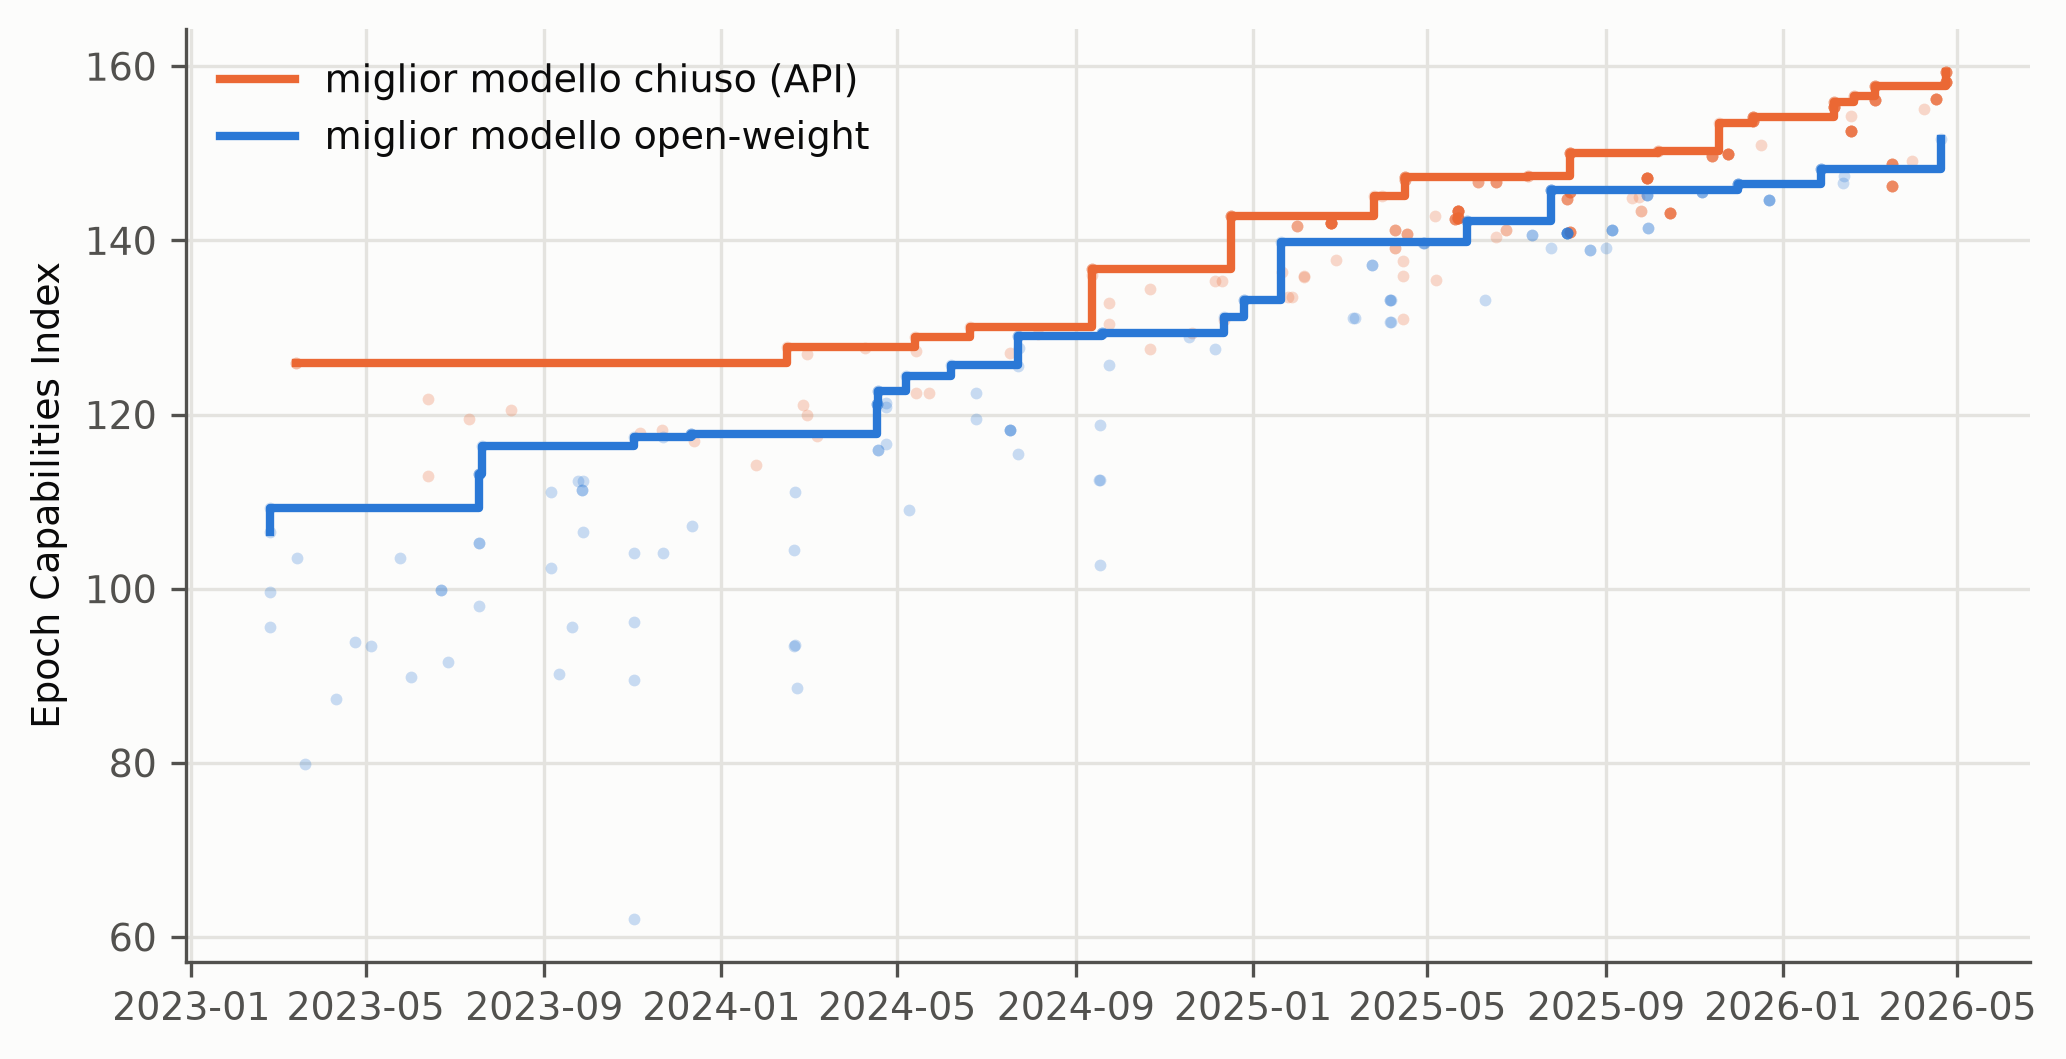
\includegraphics[width=\textwidth]{images/locality/open_closed_gap.png}
\caption{Capacità del miglior modello chiuso e del miglior modello open-weight nel tempo, sull'indice aggregato di
capacità di Epoch AI (punti: singoli modelli; linee: migliore fino a quel momento). Grafico ricavato dalla tabella dati
pubblicata da Epoch AI~\cite{epoch2026openclosed}.}
\label{fig:local-gap}
\end{figure}

Per un dispositivo personale non conta il miglior modello aperto, che può avere centinaia di miliardi di parametri, ma il
miglior modello che entra in un hardware consumer. Epoch AI misura direttamente questa grandezza. Considerando i modelli
abbastanza piccoli da girare su una singola scheda grafica consumer, al massimo circa 28 miliardi di parametri per una
scheda da 24\,GB e circa 40 miliardi per una da 32\,GB, rileva che su quattro benchmark essi raggiungono le prestazioni
del modello di frontiera del momento dopo sei-dodici mesi~\cite{epoch2025consumergpu}. Tre forze trainano il recupero:
gli sviluppatori di modelli aperti aumentano il calcolo di addestramento più o meno alla stessa velocità di quelli
chiusi, la distillazione, cioè l'addestramento di un modello piccolo a imitare le risposte di uno grande, ne trasferisce gran
parte delle capacità, e ogni nuova
generazione di schede grafiche aumenta la dimensione dei modelli che vi trovano posto~\cite{epoch2025bestmodel}. La
stessa tendenza emerge dal lato opposto: il modello più piccolo con un punteggio superiore al 60\,\% sul benchmark MMLU, un
insieme di domande a scelta multipla su 57 materie, aveva 540 miliardi di parametri nel 2022 e 3.8 miliardi nel 2024, una riduzione di 142 volte~\cite{stanford2025aiindex}.

\subsection{Small language model}
\label{sec:local-slm}

All'estremo inferiore della scala si trovano gli \emph{small language model}. Le definizioni variano; una rassegna che ne
misura diverse decine sui dispositivi colloca l'intervallo tra 100 milioni e 5 miliardi di parametri, con architettura
decoder-only, cioè quella dei comuni LLM che generano il testo da sinistra a destra~\cite{lu2024slm}. I modelli piccoli
vengono addestrati su molti più dati di quanto converrebbe se si volesse soltanto minimizzare il costo
dell'addestramento. Il motivo è che per essi il costo che conta è l'inferenza, ripetuta milioni di volte dopo
l'addestramento: conviene quindi spendere di più una volta sola per ottenere un modello piccolo ma capace. Un modello da
mezzo miliardo di parametri può così vedere migliaia di miliardi di token~\cite{lu2024slm}. Misurati su dispositivi edge con pesi a 4 bit, i modelli tra 0.1 e 3 miliardi di parametri
richiedono tra 0.3 e 2.5\,GB di memoria, e con contesti lunghi la maggior parte della memoria è occupata dalla KV cache, che conserva il contesto già letto
(Sezione~\ref{sec:local-phases}), e dai buffer di calcolo~\cite{lu2024slm}. Le ricerche sui modelli sotto il miliardo di parametri sostengono che, sugli smartphone,
un'applicazione non dovrebbe usare più di circa un decimo della memoria del dispositivo, e mostrano che un modello da 350
milioni di parametri progettato con cura eguaglia un modello generalista da 7 miliardi su un task ristretto come
l'invocazione di un'interfaccia applicativa~\cite{liu2024mobilellm}.

I produttori di piattaforme hanno adottato la stessa idea. Il foundation model che Apple impiega sui propri dispositivi
ha circa tre miliardi di parametri, è quantizzato a meno di quattro bit per peso ed è specializzato per ciascuna
funzionalità con piccoli adapter low-rank, moduli aggiuntivi con pochi parametri addestrati sul singolo compito
(Sezione~\ref{sec:bg-peft})~\cite{gunter2024apple}; la famiglia Gemma~3n di Google è progettata per girare
su smartphone e laptop con un'impronta di memoria ridotta, ed è promossa esplicitamente per la privacy e l'uso
offline~\cite{google2025gemma3n}. GroundOne segue lo stesso schema: un modello open-weight piccolo, quantizzato e
specializzato da un adapter per un unico task.

\section{Il costo dell'inferenza su un singolo dispositivo}
\label{sec:bg-inference}

Le sezioni precedenti spiegano perché un modello dovrebbe girare in locale e quali modelli possono farlo. Questa sezione
spiega quanto costa eseguirne uno, e perché il costo dipende così tanto da ciò che gli si chiede di fare.

\subsection{Prefill e decoding}
\label{sec:local-phases}

Un modello linguistico decoder-only elabora una richiesta in due fasi. Nella fase di \emph{prefill} legge l'intero prompt
in una volta. Per farlo usa il meccanismo di attenzione, con cui ogni token raccoglie informazioni dai token che lo
precedono: ogni strato calcola, per ciascun token di input, due vettori (una \emph{chiave} e un \emph{valore}) che i
token successivi consulteranno, e li memorizza nella \emph{KV cache} (dall'inglese key-value). Nella fase di \emph{decoding} produce l'output un token alla
volta; ogni nuovo token consulta la cache attraverso l'attenzione e la estende di una posizione~\cite{pope2023scaling}. Il
prefill elabora molti token in parallelo, il decoding uno solo. I sistemi che servono i modelli a molti utenti sfruttano questa differenza in vari
modi, per esempio gestendo la cache a pagine per accogliere più richieste concorrenti~\cite{kwon2023pagedattention}
oppure eseguendo le due fasi su macchine diverse, ciascuna adatta alla propria~\cite{patel2024splitwise}.

La conseguenza è visibile sul laptop usato in questa tesi (Figura~\ref{fig:local-prefill-decode}). Con il modello da
0.5B, leggere un token del prompt richiede meno di 0.4 millisecondi, mentre scrivere un token di output ne richiede 5.9,
sedici volte di più. Con il modello da 3B i valori sono 2.2 e 31.8 millisecondi, quattordici volte di più. Un modello
che scrive un breve paragrafo impiega quindi più tempo a scriverlo che a leggere un documento di diverse migliaia di
token.

\begin{figure}[htbp]
\centering
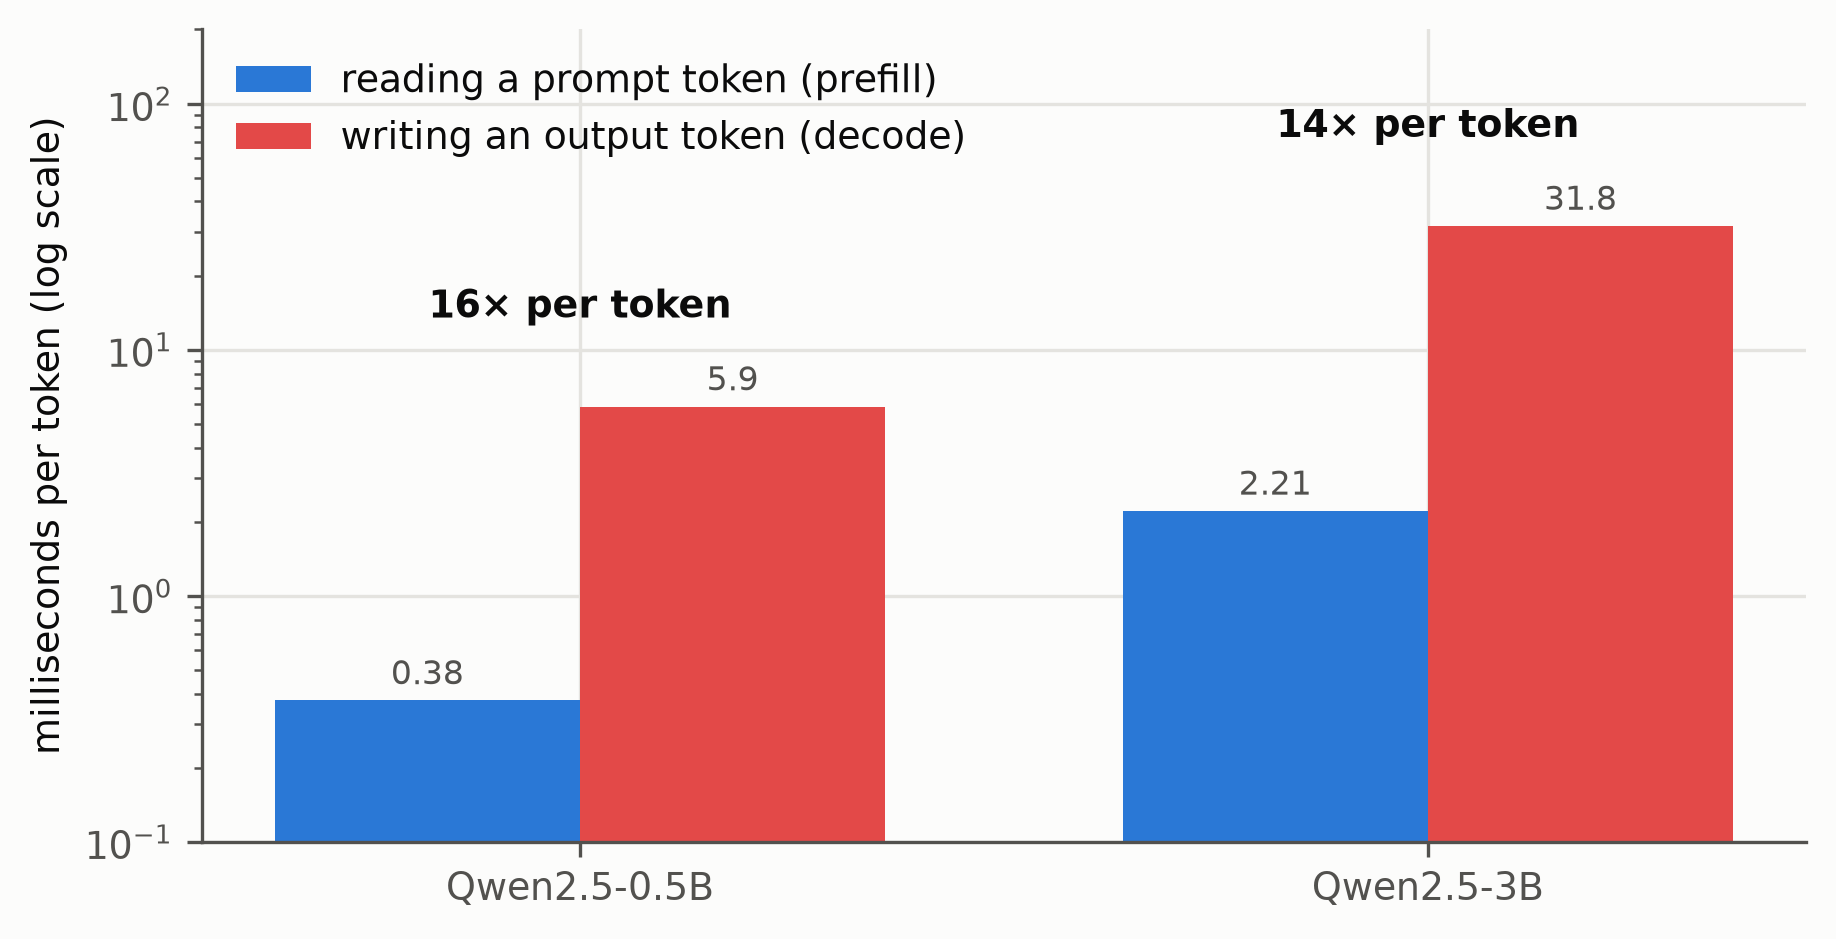
\includegraphics[width=0.85\textwidth]{images/locality/prefill_vs_decode_m4.png}
\caption{Tempo per token quando il modello legge l'input (prefill) e quando scrive l'output (decoding), misurato sulla
macchina della tesi (Apple M4, 16\,GB, MLX a 8 bit, una richiesta alla volta). Prefill: mediana su contesti di 500, 1000 e 2000 token.}
\label{fig:local-prefill-decode}
\end{figure}

\subsection{Il modello roofline}
\label{sec:local-roofline}

La ragione di questa asimmetria è colta dal modello roofline, un semplice modello delle prestazioni introdotto per i
processori multicore~\cite{williams2009roofline}. Una computazione è caratterizzata dalla sua \emph{intensità
aritmetica}, cioè dal numero di operazioni in virgola mobile che esegue per ogni byte letto dalla memoria. Un processore
ha due limiti: una velocità di calcolo di picco e una banda di memoria di picco. La velocità raggiungibile è il minimo
tra il calcolo di picco e il prodotto tra banda e intensità. Una computazione a bassa intensità è limitata dalla banda,
una ad alta intensità dal calcolo; l'intensità alla quale i due limiti si incontrano si chiama punto di cresta (ridge
point)~\cite{williams2009roofline}.

Applicato a un transformer, il modello separa nettamente le due fasi~\cite{yuan2024unveiled}. Ogni matrice di pesi di uno
strato lineare deve essere letta dalla memoria una volta per forward pass. Durante il prefill la stessa matrice
moltiplica gli stati nascosti di centinaia o migliaia di token, quindi ogni byte di pesi serve per centinaia di
operazioni: l'intensità è alta e il limite è il calcolo. Durante il decoding la matrice moltiplica un singolo vettore,
quindi ogni peso serve per circa due operazioni: l'intensità è vicina a uno e il limite è la banda. Per un modello da 7
miliardi di parametri a 16 bit, gli strati lineari raggiungono intensità superiori a mille operazioni per byte nel
prefill e di circa una nel decoding~\cite{yuan2024unveiled}. Nei datacenter questo squilibrio si attenua: il decoding di
molte richieste contemporanee viene raggruppato in batch, così che ogni peso letto dalla memoria serve a generare più
token e l'intensità sale~\cite{pope2023scaling}. Un dispositivo personale serve invece un solo utente, una richiesta alla
volta, e non può contare su questo rimedio: è qui che l'asimmetria tra le due fasi pesa di più.

La Figura~\ref{fig:local-roofline} traccia il roofline della macchina della tesi. Apple pubblica la banda di memoria,
120\,GB/s, ma non la velocità di calcolo di picco~\cite{apple2024m4specs}; il tetto piatto della figura è quindi la
velocità effettivamente raggiunta durante il prefill, circa 2.8 TFLOP/s, che costituisce
un limite inferiore del picco. Il ridge point si trova a circa 23 operazioni per byte. La generazione di un token si
colloca a circa due operazioni per byte, un ordine di grandezza sotto il ridge point, mentre la lettura di un documento
di centinaia di token si colloca un ordine di grandezza sopra. Le due fasi dello stesso modello, sulla stessa macchina,
vivono in regimi diversi.

\begin{figure}[htbp]
\centering
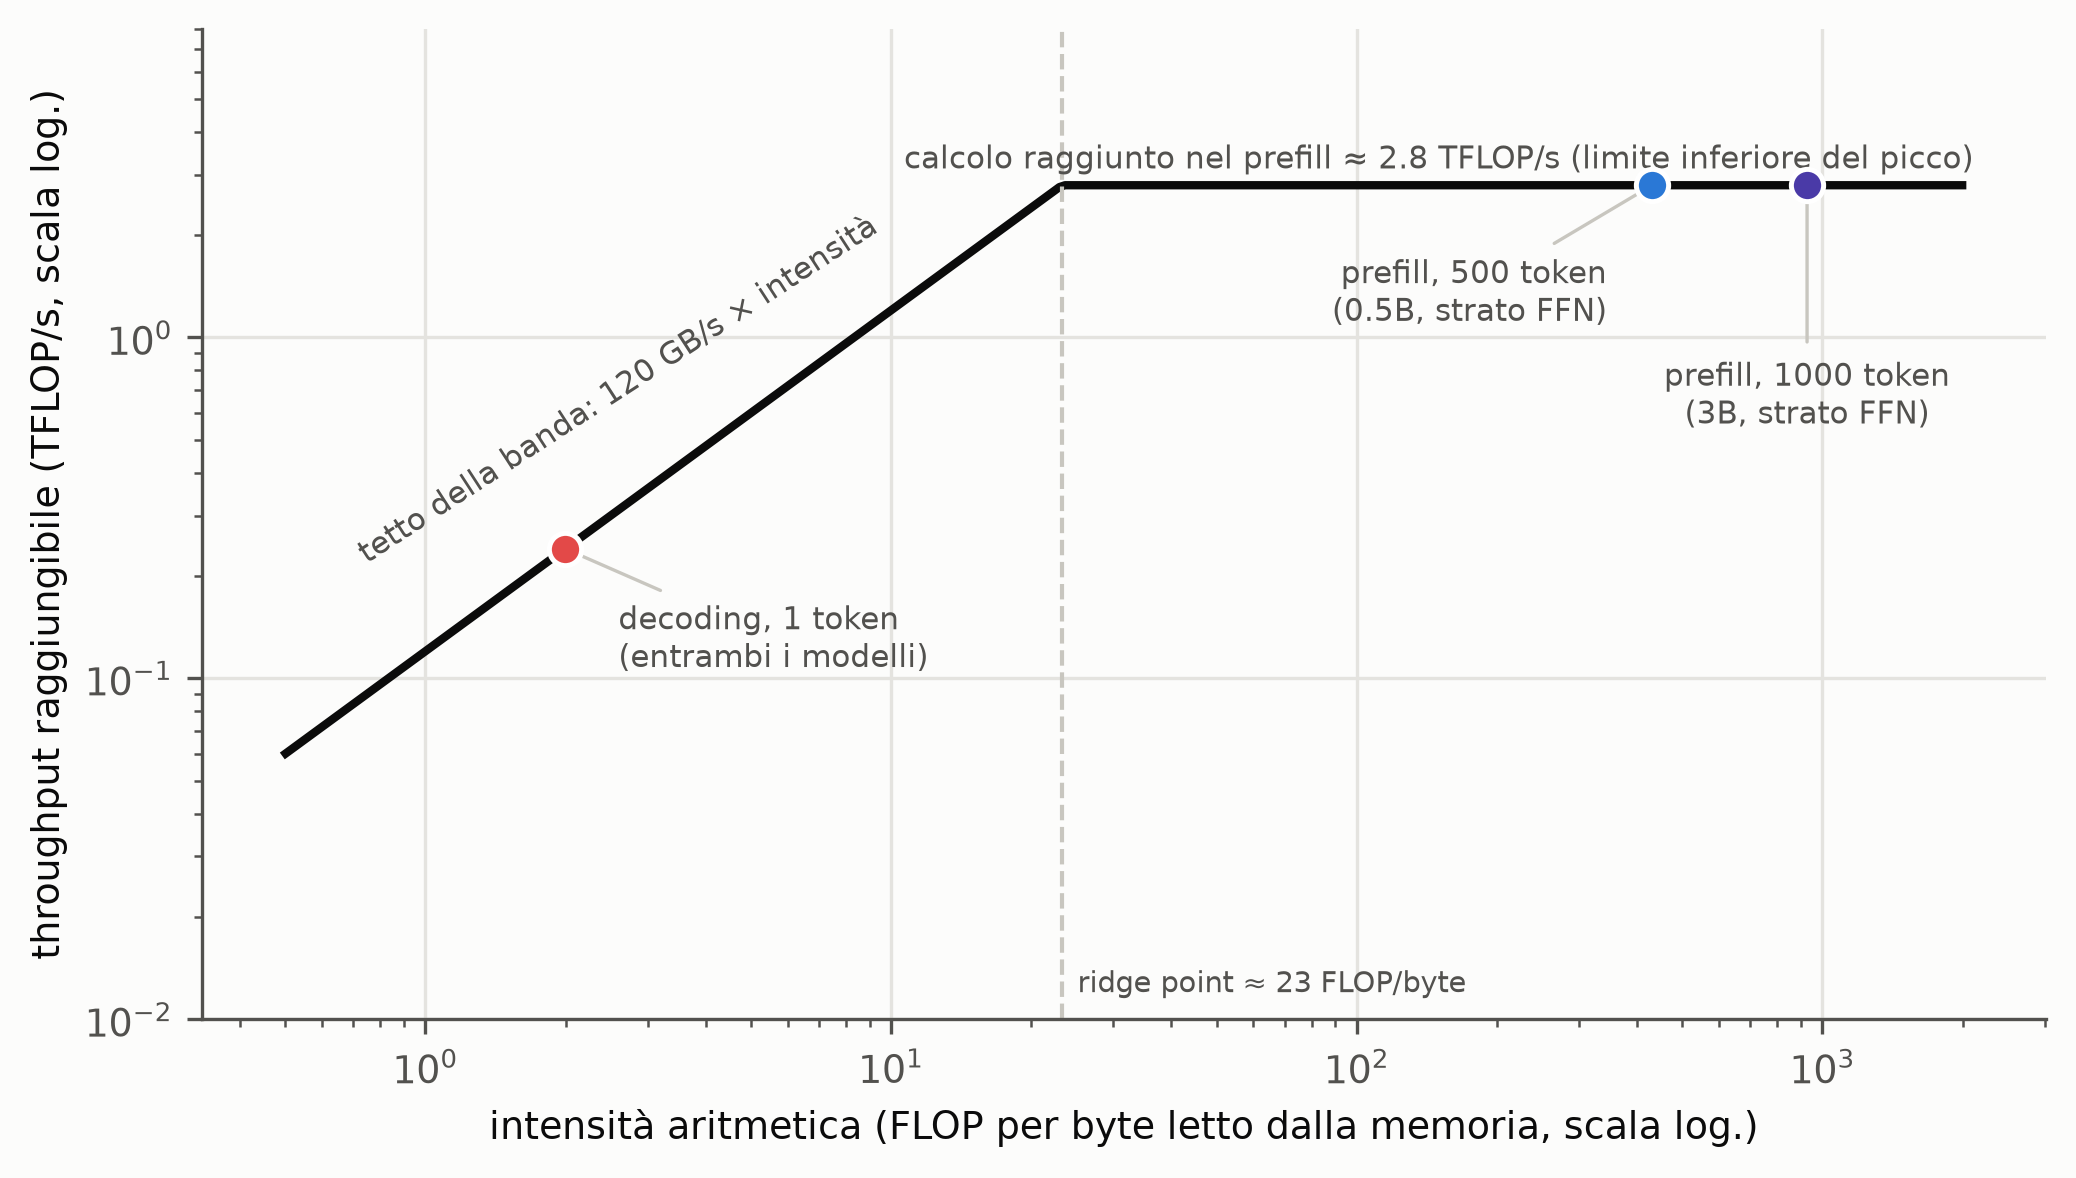
\includegraphics[width=\textwidth]{images/locality/roofline_m4.png}
\caption{Modello roofline della macchina della tesi~\cite{williams2009roofline}. Tetto inclinato: banda di memoria
dichiarata da Apple (120\,GB/s). Tetto piatto: throughput raggiunto nel prefill, limite inferiore del picco non
pubblicato. Intensità calcolate per uno strato feed-forward di Qwen2.5 con pesi a 8 bit e attivazioni a 16 bit;
l'attenzione è trascurata.}
\label{fig:local-roofline}
\end{figure}

\subsection{Un limite inferiore alla generazione}
\label{sec:local-floor}

Poiché il decoding legge ogni peso una volta per ogni token generato, il suo tempo per token non può scendere sotto la
dimensione dei pesi divisa per la banda di memoria, qualunque sia l'hardware. Per il modello da 3B a 8 bit, i cui pesi
occupano circa 3.3\,GB, questo limite vale 27 millisecondi per token su una macchina da 120\,GB/s; i 31.8 millisecondi
misurati lo superano solo di circa un sesto. Il limite dipende da due soli numeri, la dimensione del modello e la banda
della macchina, e si applica a ogni modello che genera testo. È la chiave per confrontare l'hardware nella
Sezione~\ref{sec:local-hardware} e per la conseguenza tratta nella Sezione~\ref{sec:local-verification}.

La capacità di memoria impone un secondo limite, ancora più rigido: i pesi devono entrare in memoria. Un modello richiede
circa due byte per parametro nel formato a 16 bit usato in addestramento, uno a 8 bit e mezzo a 4 bit, più alcuni piccoli
fattori di scala per ogni gruppo di pesi, necessari a ricostruirne il valore (Figura~\ref{fig:local-memory}). Un modello da 7 miliardi di parametri a 16 bit richiede 14\,GB per i soli
pesi, più di quanto la maggior parte dei dispositivi personali possa mettere a disposizione~\cite{alizadeh2024flash}; a 4
bit ne richiede circa 4. A questi si aggiungono la KV cache, le attivazioni, il sistema operativo e ogni altro modello in
esecuzione nello stesso momento. Un laptop da 16\,GB può quindi ospitare un generatore da 7--8 miliardi di parametri a 4
bit accanto a un piccolo verificatore, ma non molto di più.

\begin{figure}[htbp]
\centering
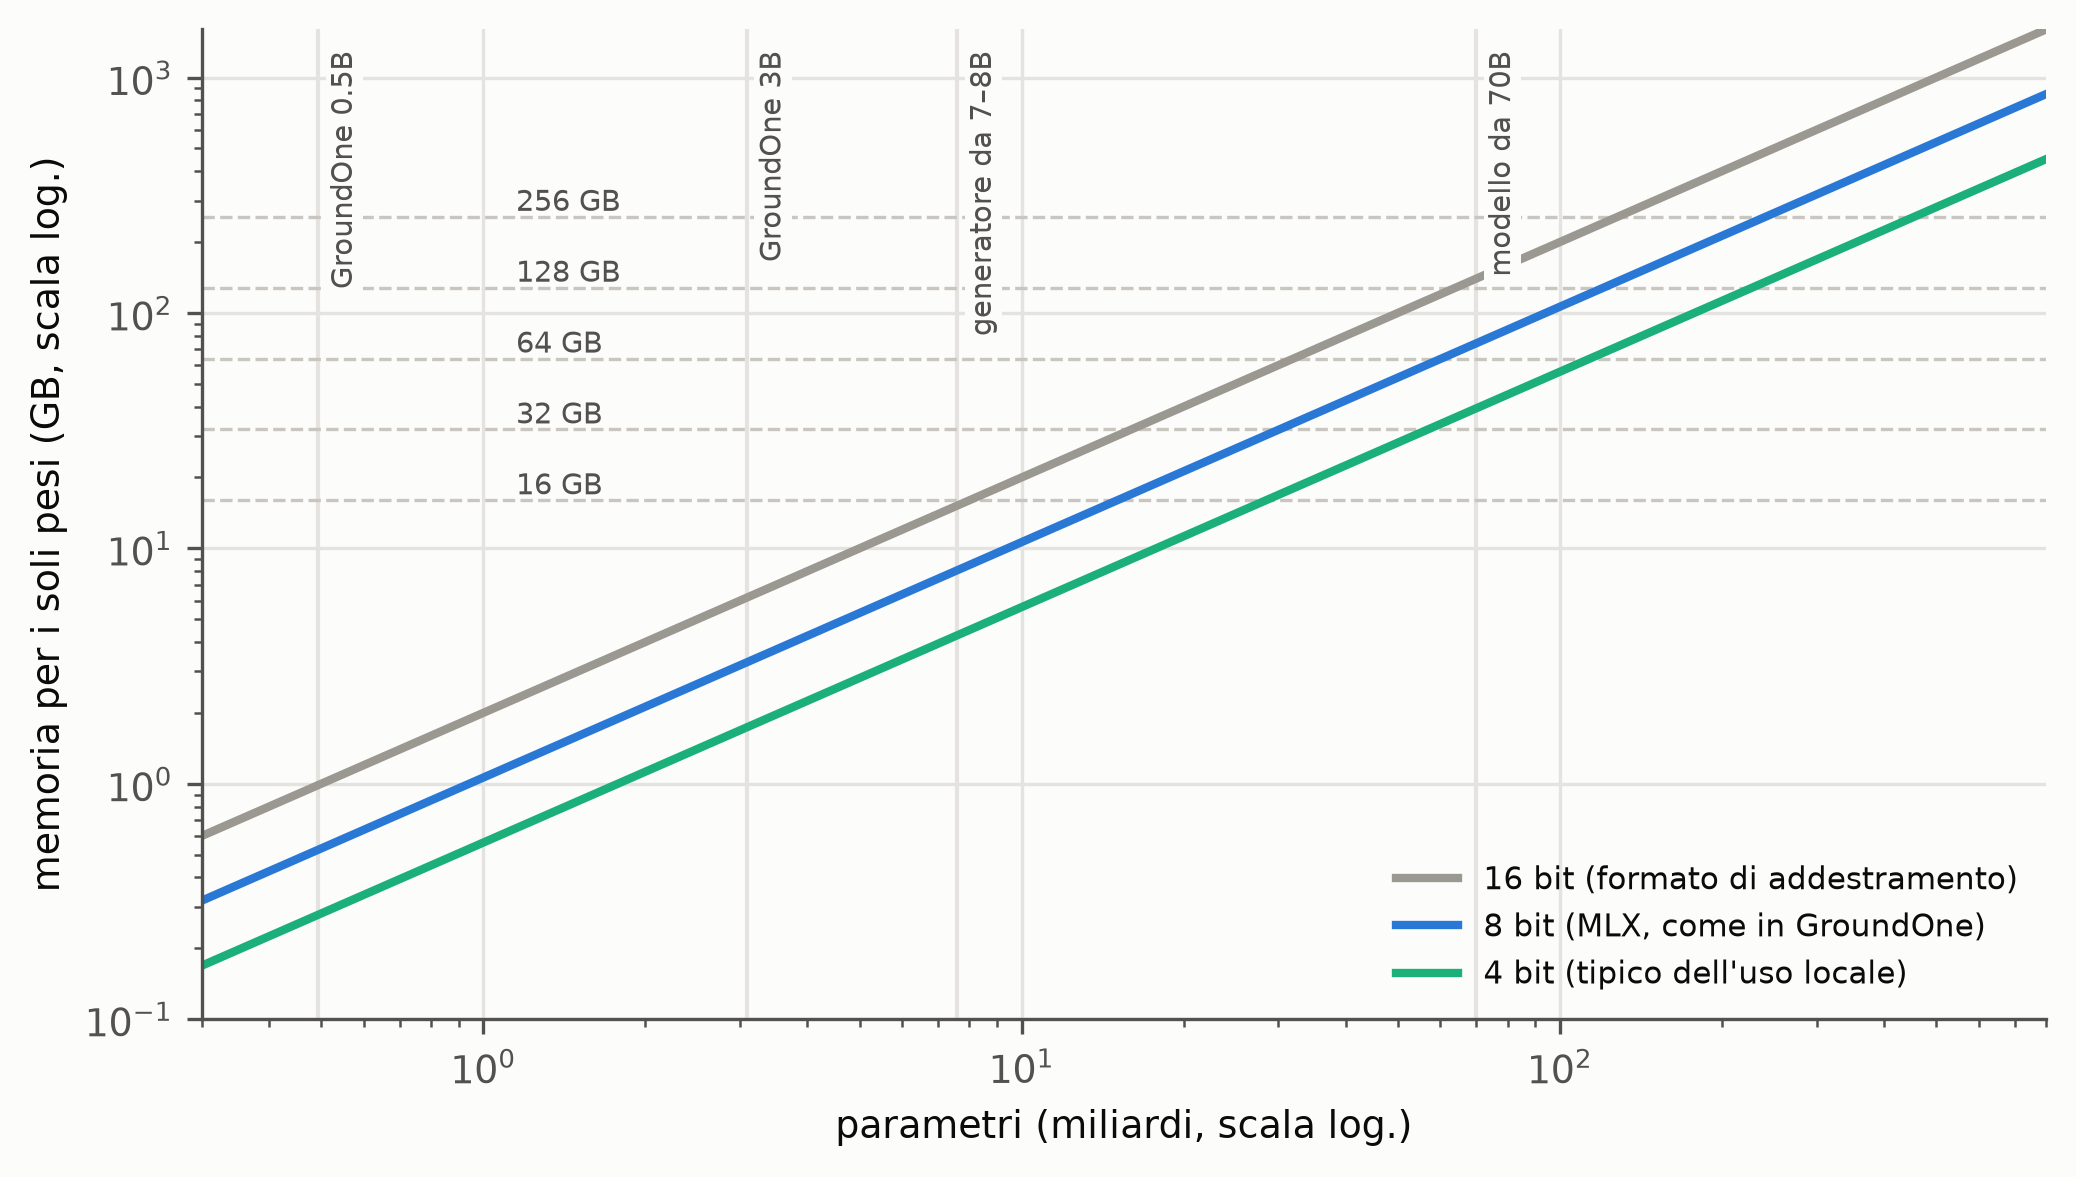
\includegraphics[width=\textwidth]{images/locality/memory_fit.png}
\caption{Memoria necessaria per i pesi di un modello in funzione della sua dimensione e della precisione (numero di parametri
moltiplicato per i bit per peso, compreso mezzo bit di scale per gruppo nei formati quantizzati). Linee tratteggiate: tagli di memoria
comuni nell'hardware locale. La KV cache, le attivazioni e gli altri modelli in esecuzione si aggiungono a questo valore.}
\label{fig:local-memory}
\end{figure}

\section{L'hardware per l'inferenza locale}
\label{sec:local-hardware}

Il modello di costo riduce la scelta dell'hardware per l'inferenza locale a tre grandezze. La \emph{capacità di memoria}
stabilisce quali modelli entrano. La \emph{banda di memoria} stabilisce quanto velocemente possono generare. La
\emph{capacità di calcolo} stabilisce quanto velocemente possono leggere. Potenza e prezzo completano il quadro. Questa
sezione passa in rassegna l'hardware disponibile a ottobre 2026 lungo questi assi, sulla base delle specifiche pubblicate
dai produttori.

\subsection{Classi di hardware}
\label{sec:local-classes}

Dominano due architetture. In un sistema \emph{discreto} la scheda grafica ha una propria memoria, veloce ma piccola, e
il modello deve entrare in essa. In un sistema a \emph{memoria unificata} il processore e l'unità grafica condividono un
unico, ampio blocco di memoria, così che un modello può usarne la maggior parte, con una banda però inferiore a quella di
una scheda grafica di fascia alta. I processori di Apple, il DGX Spark di NVIDIA e il Ryzen AI Max (Strix Halo) di AMD
seguono tutti questa seconda architettura. La Figura~\ref{fig:local-memarch} mette a confronto le due architetture.

\begin{figure}[htbp]
\centering
\subfloat[Sistema discreto: la GPU legge i pesi dalla propria VRAM, molto veloce ma limitata a 16--32\,GB; il resto del
sistema è raggiungibile solo attraverso il PCIe.]{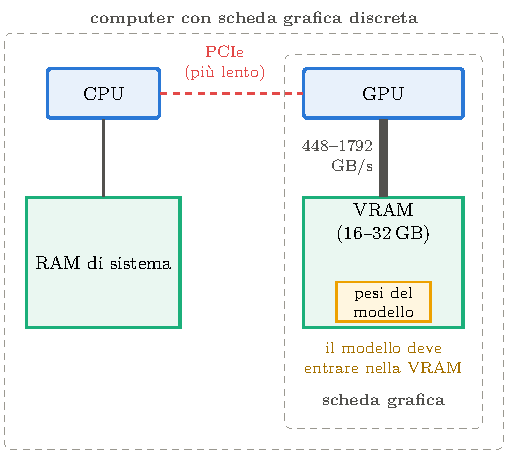
\includegraphics[width=0.53\textwidth]{images/diagrams/memory_discrete_tikz.pdf}\label{fig:local-memarch-discrete}}\hfill
\subfloat[Memoria unificata: CPU, GPU e NPU sullo stesso chip condividono un unico blocco di memoria, più ampio ma con
una banda inferiore.]{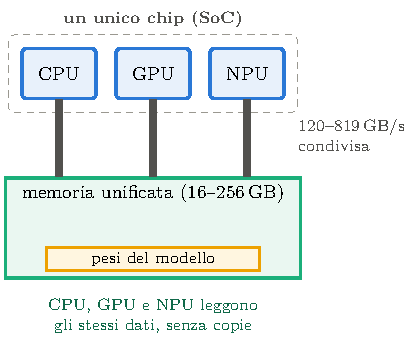
\includegraphics[width=0.43\textwidth]{images/diagrams/memory_unified_tikz.pdf}\label{fig:local-memarch-unified}}
\caption{Le due architetture dell'hardware per l'inferenza locale. Rettangoli blu: unità di calcolo; rettangoli verdi:
memoria; rettangolo arancione: i pesi del modello; spessore delle linee: banda indicativa. Valori di capacità e banda
dalla Tabella~\ref{tab:local-hardware}. In un sistema discreto un modello che non entra nella VRAM deve passare dal
collegamento PCIe, molto più lento; in un sistema a memoria unificata il modello può occupare quasi tutta la memoria della
macchina, ma ogni token generato la legge a una velocità inferiore a quella di una scheda grafica di fascia alta.}
\label{fig:local-memarch}
\end{figure} La Tabella~\ref{tab:local-hardware} e la Figura~\ref{fig:local-hardware}
collocano le principali opzioni sui due assi della memoria. La Figura~\ref{fig:local-photos} mostra
alcuni dei sistemi citati, per dare un'idea concreta di come si presentano.

\begin{figure}[htbp]
\centering
\subfloat[MacBook Pro da 14 pollici con M4, la macchina della tesi.]{
\includegraphics[width=0.31\textwidth]{images/hardware/macbook_pro_m4.png}}\hfill
\subfloat[Mac mini (2024, M4).]{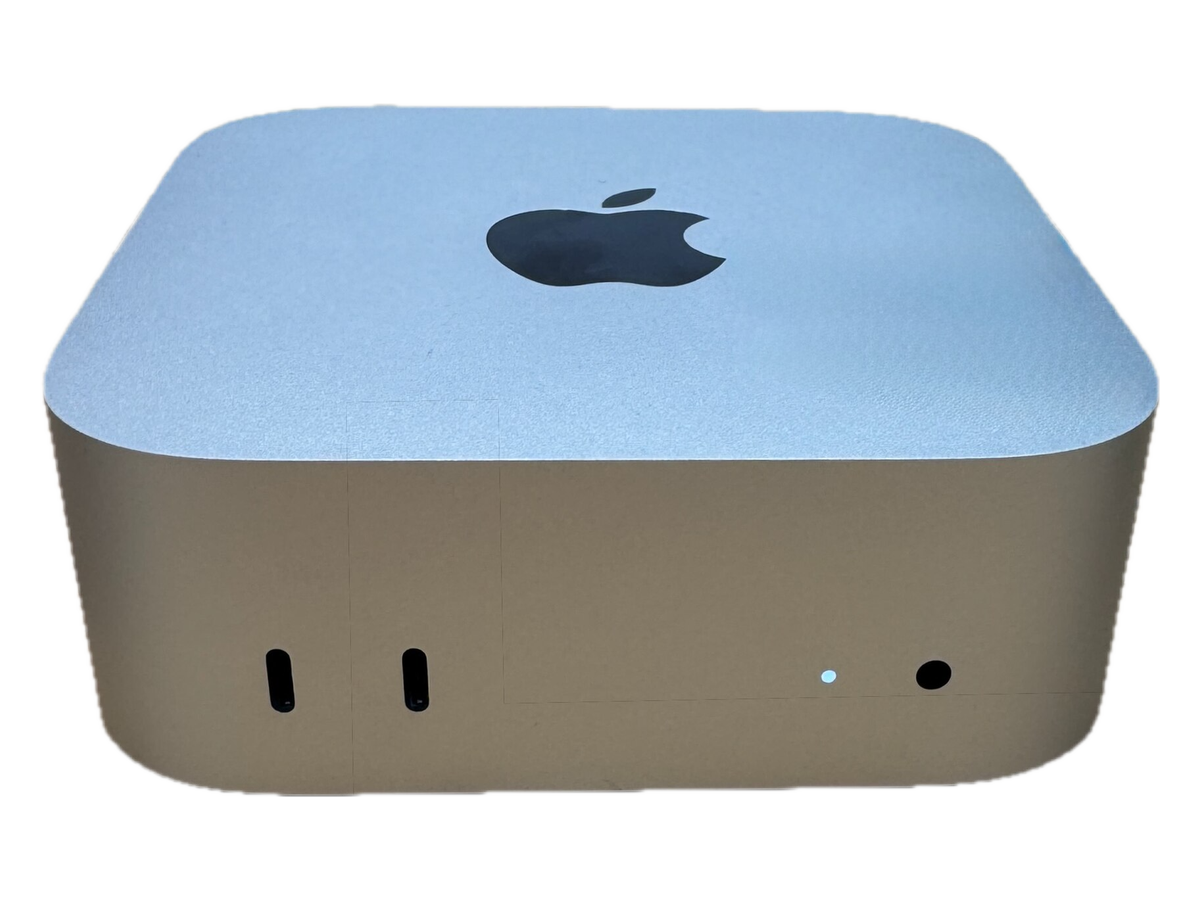
\includegraphics[width=0.31\textwidth]{images/hardware/mac_mini_m4.png}}\hfill
\subfloat[Mac Studio.]{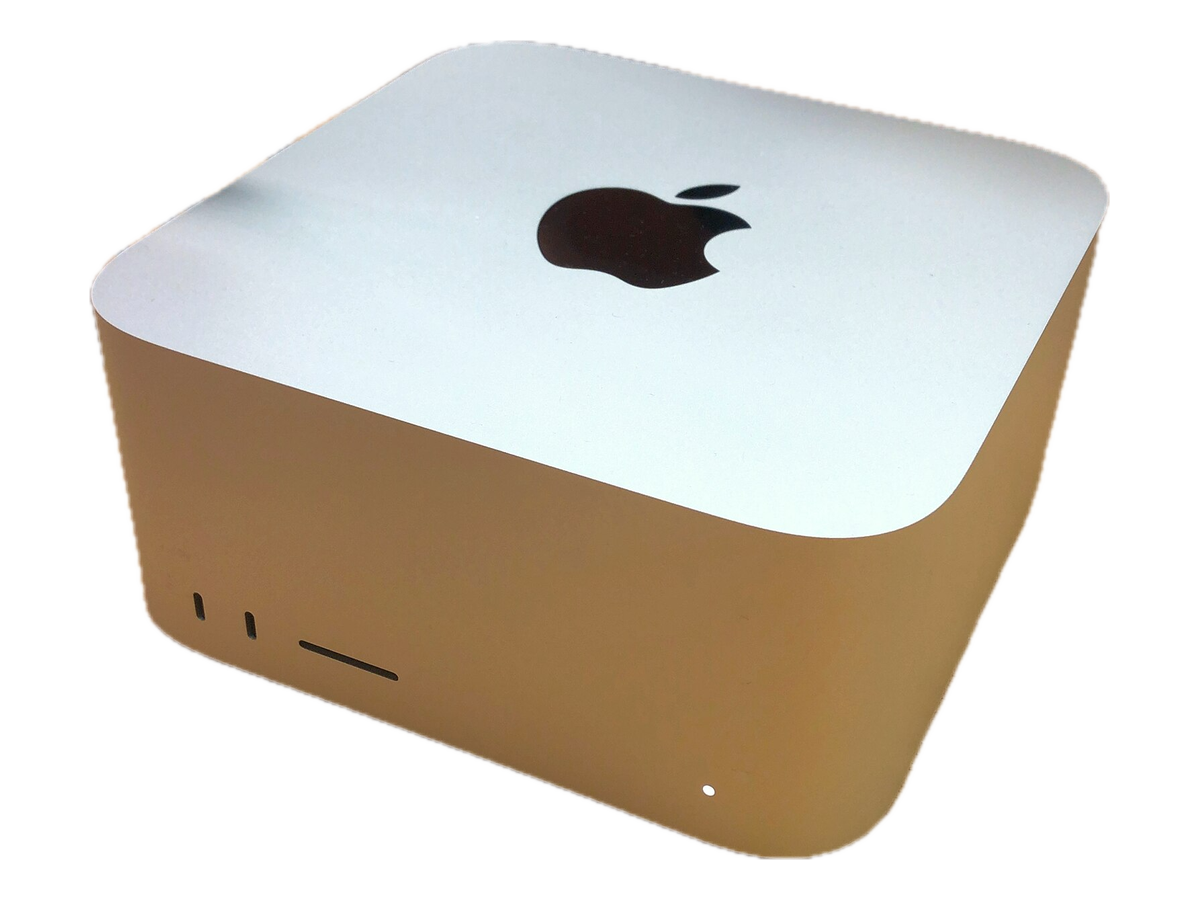
\includegraphics[width=0.31\textwidth]{images/hardware/mac_studio.png}}\\[0.6em]
\subfloat[NVIDIA DGX Spark.]{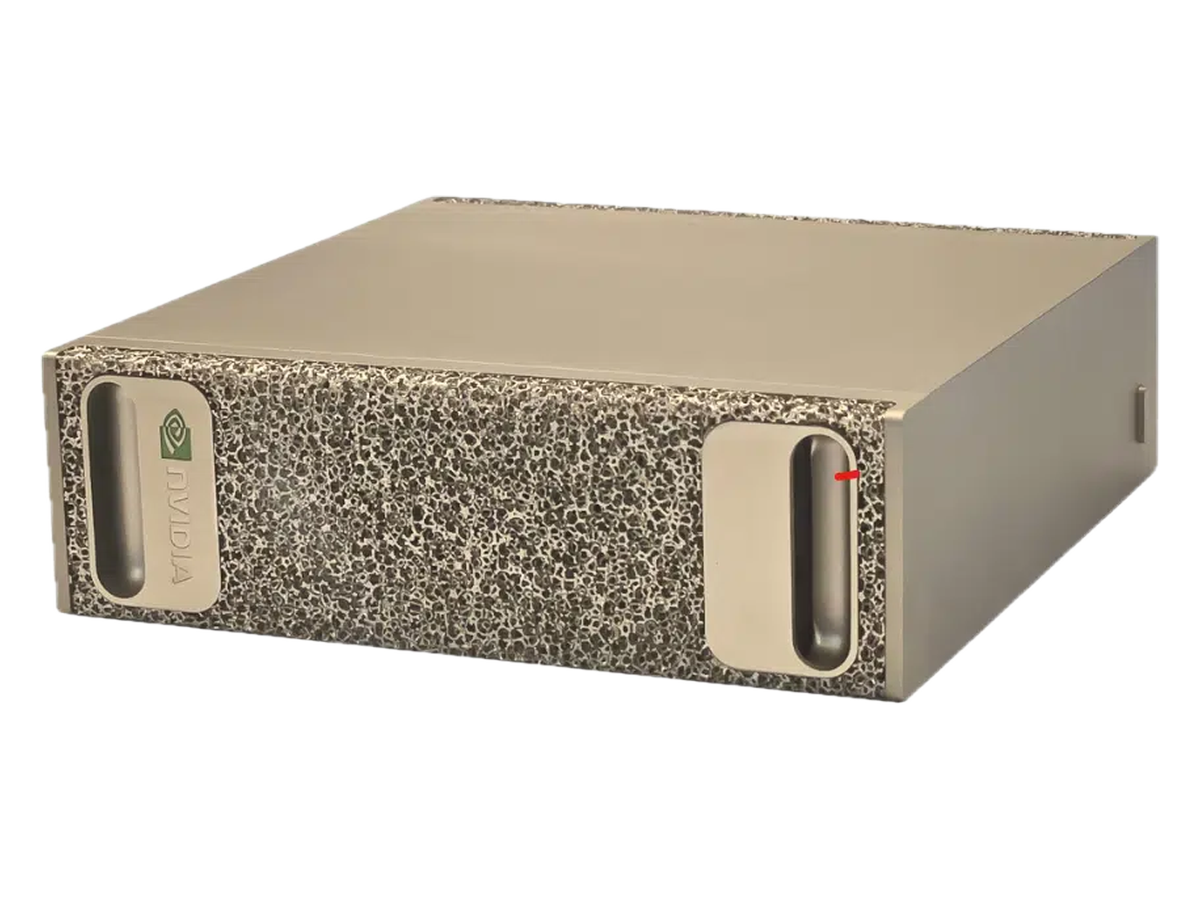
\includegraphics[width=0.31\textwidth]{images/hardware/dgx_spark.png}}\hspace{0.035\textwidth}
\subfloat[Scheda grafica GeForce RTX 5090 Founders Edition.]{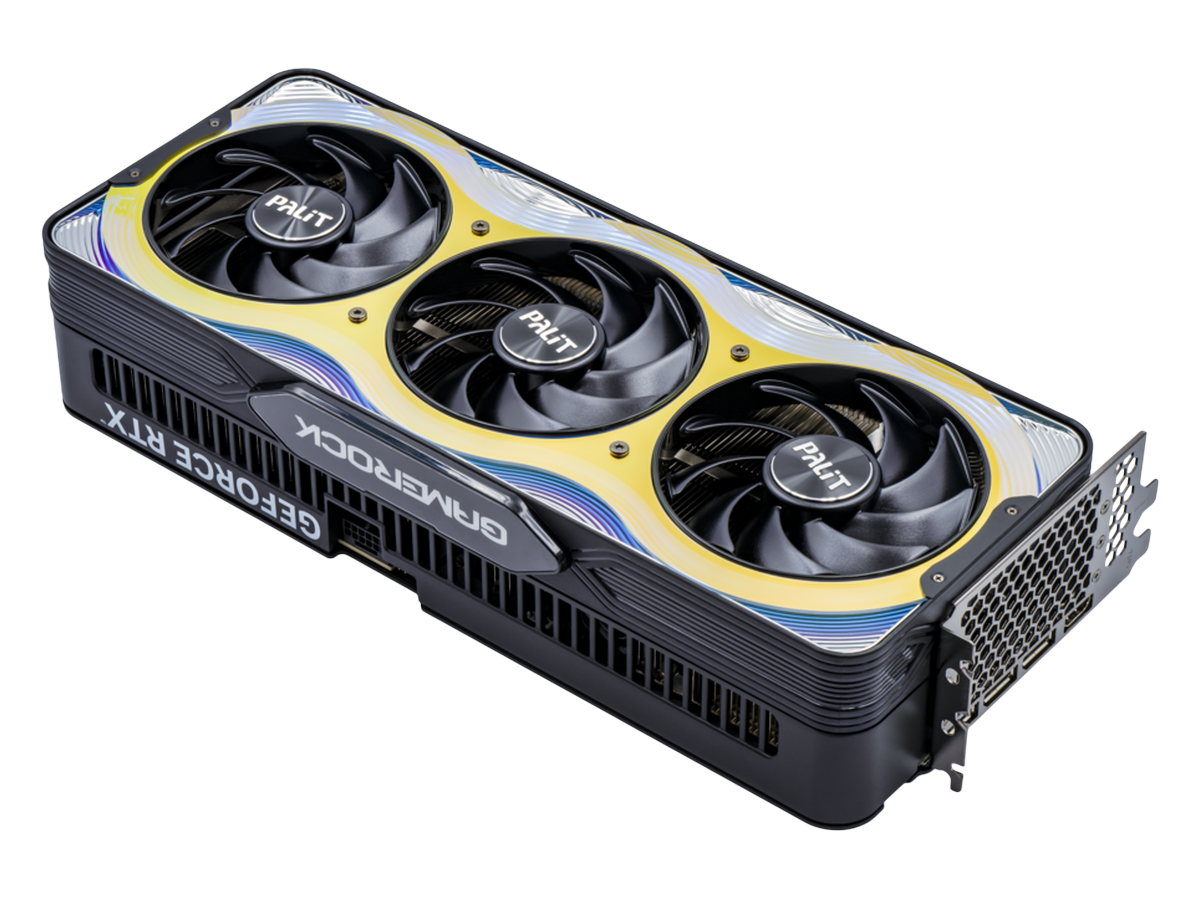
\includegraphics[width=0.31\textwidth]{images/hardware/rtx_5090.png}}
\caption{Alcuni dei sistemi per l'inferenza locale confrontati in questa sezione (immagini non in scala). Fonti: (a),
(c) Apple; (b) LoMit, Wikimedia Commons, CC0; (d), (e) NVIDIA. Le immagini dei produttori sono materiale promozionale,
riprodotto a scopo di documentazione scientifica.}
\label{fig:local-photos}
\end{figure}

\begin{table}[htbp]
\centering
\caption{Hardware per l'inferenza locale: specifiche pubblicate dai produttori (consultate l'11 ottobre 2026). Memoria:
intervallo delle configurazioni offerte; banda: relativa a quelle configurazioni; n.d.: non dichiarato dalla fonte.}
\label{tab:local-hardware}
\small
\begin{tabularx}{\textwidth}{@{}Xrrll@{}}
\toprule
Sistema & Memoria (GB) & Banda (GB/s) & Tipo di memoria & Fonte \\
\midrule
MacBook Pro, M4 (macchina della tesi: 16\,GB) & 16--32 & 120 & unificata & \cite{apple2024m4specs} \\
MacBook Pro / Mac mini, M5 & 16--32 & 153 & unificata & \cite{apple2026mbp,apple2026macmini} \\
Mac mini, M5 Pro & 24--64 & 307 & unificata & \cite{apple2026macmini} \\
MacBook Pro, M5 Max & 36--128 & 460--614 & unificata & \cite{apple2026mbp} \\
Mac Studio, M4 Max & 36--128 & 410--546 & unificata & \cite{apple2025macstudio} \\
Mac Studio, M3 Ultra & 96--256 & 819 & unificata & \cite{apple2025macstudio} \\
NVIDIA DGX Spark (GB10) & 128 & 273 & unificata & \cite{nvidia2026dgxspark} \\
Framework Desktop, AMD Strix Halo & 32--128 (96 alla GPU) & n.d. & unificata & \cite{hachman2025framework} \\
NVIDIA RTX 5090 & 32 & 1792 & discreta & \cite{nvidia2026geforce} \\
NVIDIA RTX 5080 & 16 & 960 & discreta & \cite{nvidia2026geforce} \\
NVIDIA RTX 5060 Ti & 16 & 448 & discreta & \cite{nvidia2026geforce} \\
\bottomrule
\end{tabularx}
\end{table}

\begin{figure}[htbp]
\centering
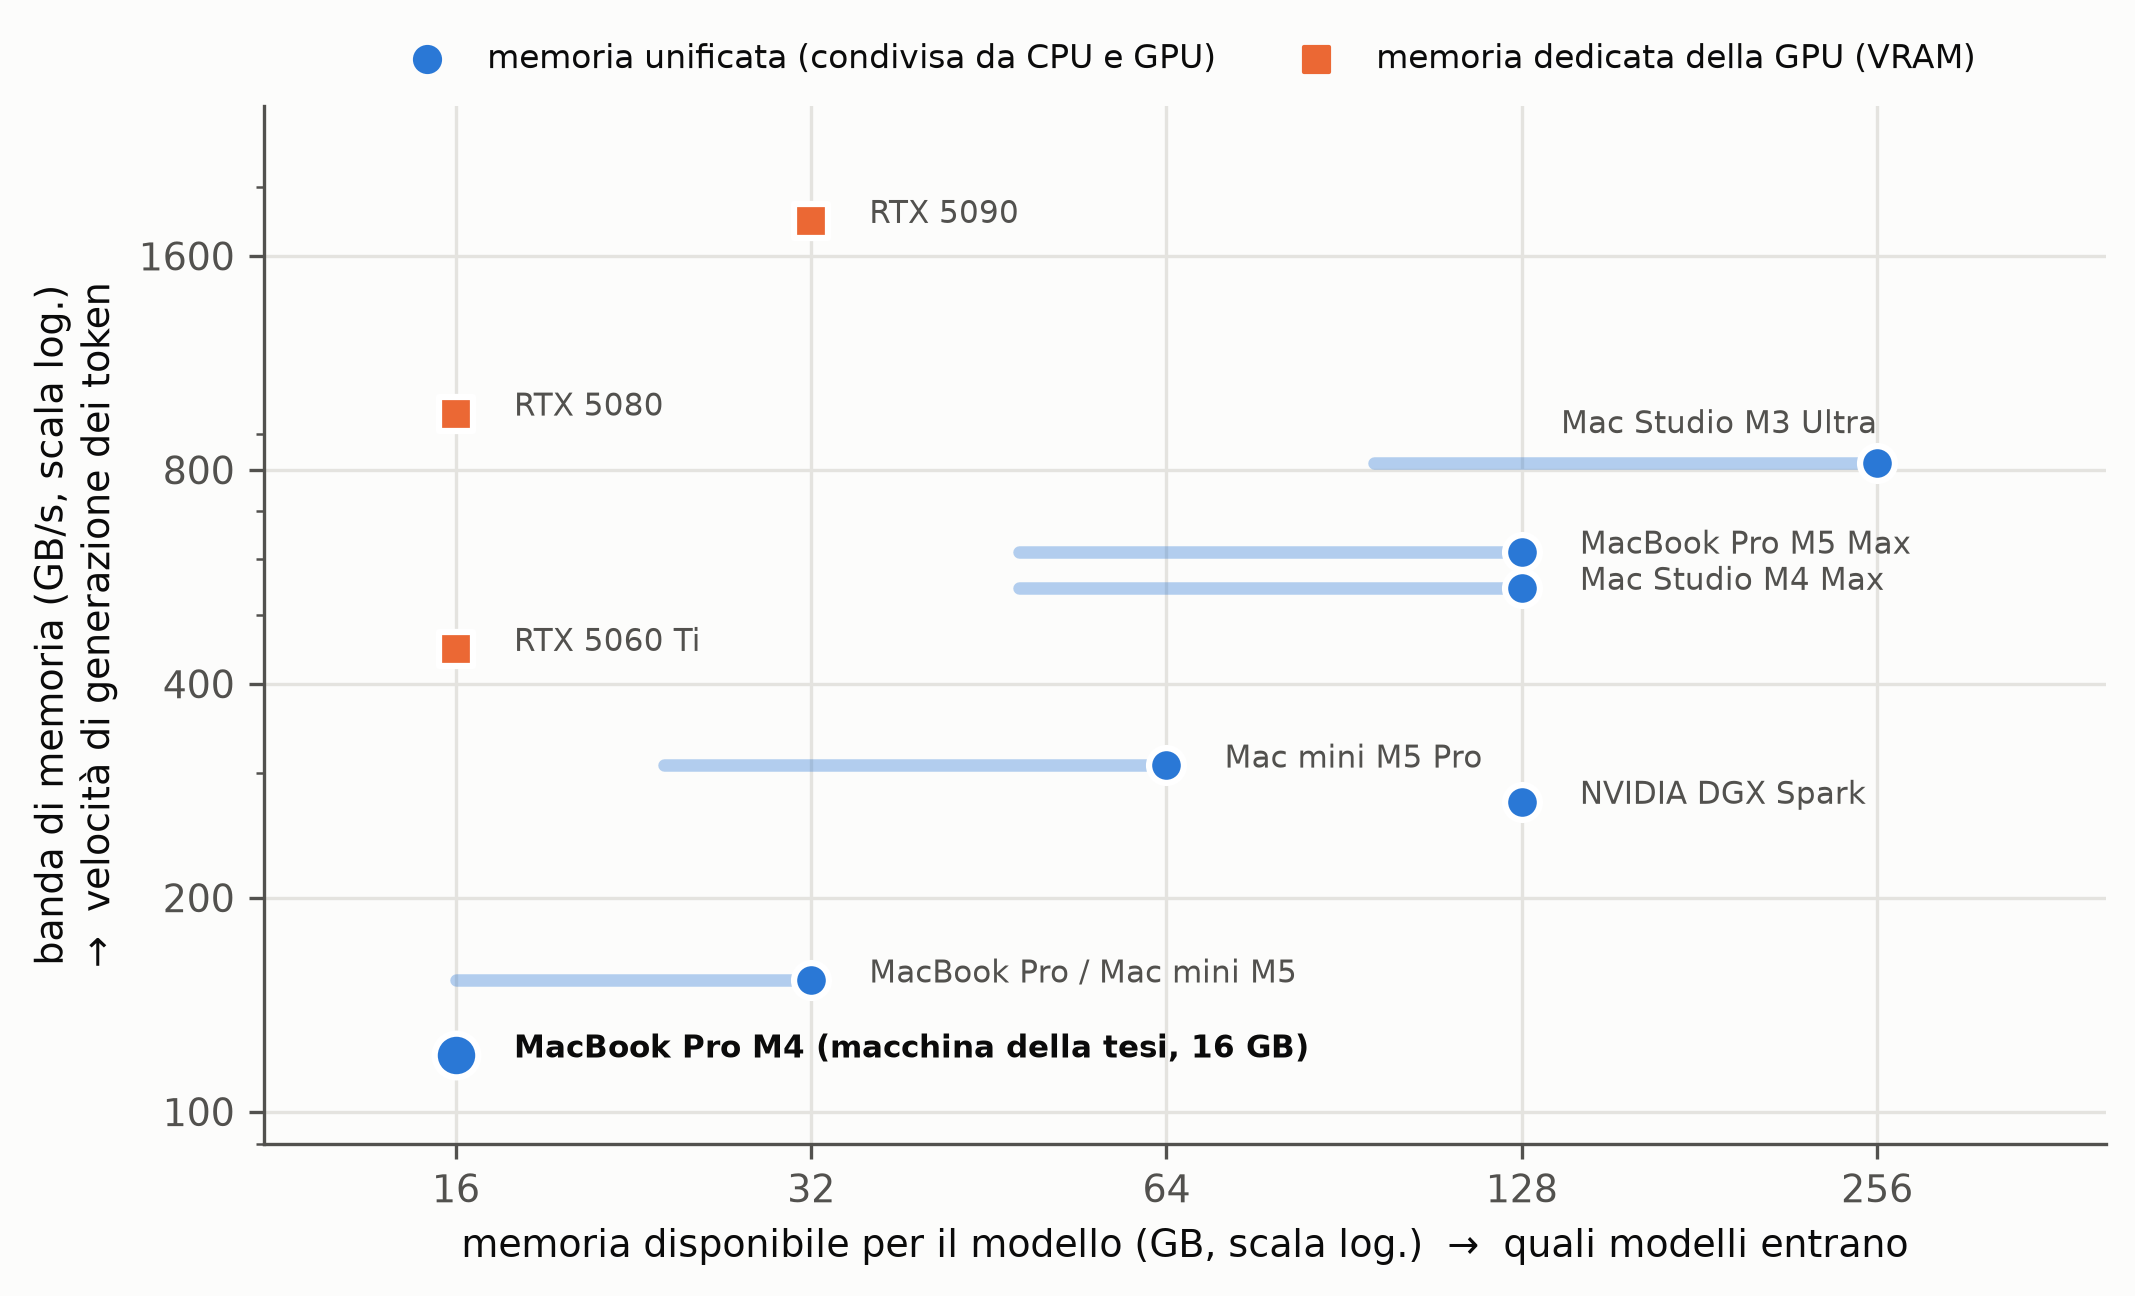
\includegraphics[width=\textwidth]{images/locality/hardware_landscape.png}
\caption{L'hardware per l'inferenza locale sui due assi che stabiliscono che cosa può girare: capacità di memoria (quali
modelli entrano) e banda di memoria (quanto velocemente si generano i token). Specifiche dei produttori: marcatori in
corrispondenza della configurazione con più memoria, barre ombreggiate sull'intervallo di tagli di memoria offerti; la
macchina della tesi è rappresentata con i suoi 16\,GB effettivi.}
\label{fig:local-hardware}
\end{figure}

\paragraph{Laptop.} I laptop con 16--32\,GB e 120--150\,GB/s, come il MacBook Pro usato in questa tesi, sono i computer
personali più diffusi su cui girano modelli locali. Ospitano senza difficoltà i modelli piccoli, e quelli da 7--8
miliardi di parametri a 4 bit. La macchina della tesi si trova in basso a sinistra nella Figura~\ref{fig:local-hardware}:
se un verificatore funziona bene lì, funziona su tutto ciò che sta sopra.

\paragraph{Macchine desktop a memoria unificata.} Una seconda classe, entro o vicino a un budget di circa tremila
dollari, offre molta più memoria con una banda moderata. Il processore Strix Halo di AMD, venduto per esempio nel
Framework Desktop, consente all'unità grafica di usare fino a 96\,GB dei suoi 128\,GB di memoria; al lancio, nell'agosto
2025, la configurazione da 128\,GB costava 1999 dollari, con una potenza del processore di 55\,W~\cite{hachman2025framework}.
Il Mac mini di Apple con M5 Pro arriva a 64\,GB a 307\,GB/s~\cite{apple2026macmini}. Macchine di questo tipo possono
ospitare modelli da decine di miliardi di parametri o modelli mixture-of-experts, composti da molte sottoreti (gli esperti) di cui ogni token ne attiva solo
una parte, così che il decoding legge soltanto i pesi degli esperti attivi, al prezzo di una generazione più lenta che su una scheda grafica.

\paragraph{Macchine dedicate all'IA.} Oltre questo budget, il Mac Studio con M3 Ultra unisce fino a 256\,GB a
819\,GB/s~\cite{apple2025macstudio}, mentre il DGX Spark di NVIDIA è un piccolo box desktop, con alimentatore da
240\,W, che contiene 128\,GB di memoria unificata con 273\,GB/s di banda e un'unità grafica Blackwell da un petaflop
($10^{15}$ operazioni al secondo) in aritmetica a 4 bit, valore che sfrutta la sparsità, cioè il salto dei pesi
nulli~\cite{nvidia2026dgxspark}. Le due macchine compiono scelte opposte, e un confronto diretto mostra il
modello di costo all'opera: su un modello da 8 miliardi di parametri con un prompt di 8000 token, il DGX Spark completa il
prefill 3.8 volte più velocemente del Mac Studio, grazie al calcolo più elevato, mentre il Mac Studio genera 3.4 volte più
velocemente, grazie a una banda tre volte superiore~\cite{exo2025spark}. Lo stesso studio combina le due macchine,
eseguendo il prefill sullo Spark e il decoding sul Mac: è la disaggregazione delle due fasi~\cite{patel2024splitwise}
portata su una scrivania.

\paragraph{Schede grafiche.} Le schede dedicate offrono di gran lunga la banda più alta, fino a 1792\,GB/s per la RTX
5090, ma al massimo 32\,GB di memoria, con una potenza di diverse centinaia di watt~\cite{nvidia2026geforce}. Sono
l'opzione più veloce per qualunque modello vi entri, e inutilizzabili per qualunque modello non vi entri.

\paragraph{Smartphone e processori mobili.} All'estremo opposto, gli smartphone hanno da 6 a 16\,GB di memoria e una
banda di qualche decina di gigabyte al secondo, condivisa da tutti i processori~\cite{li2025collaborative,xue2024powerinfer2}.
Le loro unità di elaborazione neurale (NPU) sono veloci nelle moltiplicazioni di matrici a 8 bit, e quindi nel prefill:
su uno smartphone, un modello da 7 miliardi di parametri a 4 bit legge il prompt a circa 770 token al secondo sulla NPU,
contro 37 sull'unità grafica e 8 sui core del processore~\cite{xue2024powerinfer2}. I sistemi di ricerca ne approfittano
eseguendo il prefill sulla NPU e il decoding altrove~\cite{xu2025npu}.

\subsection{L'asimmetria vale per ogni classe}
\label{sec:local-asymmetry}

Le due fasi dipendono da proprietà diverse dell'hardware, e le generazioni più recenti lo rendono esplicito. Apple
riporta che il processore M5, che aggiunge unità matriciali dedicate a ogni core grafico, riduce di 3.3--4.1 volte
rispetto all'M4 il tempo al primo token, cioè l'attesa prima che il modello inizi a rispondere, dominata dal prefill, mentre la generazione diventa soltanto 1.19--1.27 volte più
veloce, in linea con una banda di memoria passata da 120 a 153\,GB/s~\cite{apple2025m5mlx}. È la stessa Apple ad
attribuire il primo dato al calcolo e il secondo alla banda. Sui dispositivi edge, uno studio che confronta 18 coppie di
configurazioni rileva che i rallentamenti si accumulano nel decoding, mentre il tempo di valutazione del prompt varia al
massimo del 16\,\%~\cite{das2026edge}. Sugli smartphone, per i task con output breve, il prefill occupa la maggior parte
della latenza~\cite{xu2025npu}. L'hardware si sta quindi evolvendo per leggere più velocemente, molto più che per
scrivere più velocemente.

La Figura~\ref{fig:local-floor}a applica il limite inferiore della Sezione~\ref{sec:local-floor} all'hardware della
Tabella~\ref{tab:local-hardware}. Sulla scheda più veloce il modello da 3B potrebbe in linea di principio generare un
token in 1.8 millisecondi; sulla macchina della tesi il limite è di 27 millisecondi, e il tempo misurato vi si avvicina.
Un hardware migliore abbassa il limite, ma nessun hardware lo elimina.

\begin{figure}[htbp]
\centering
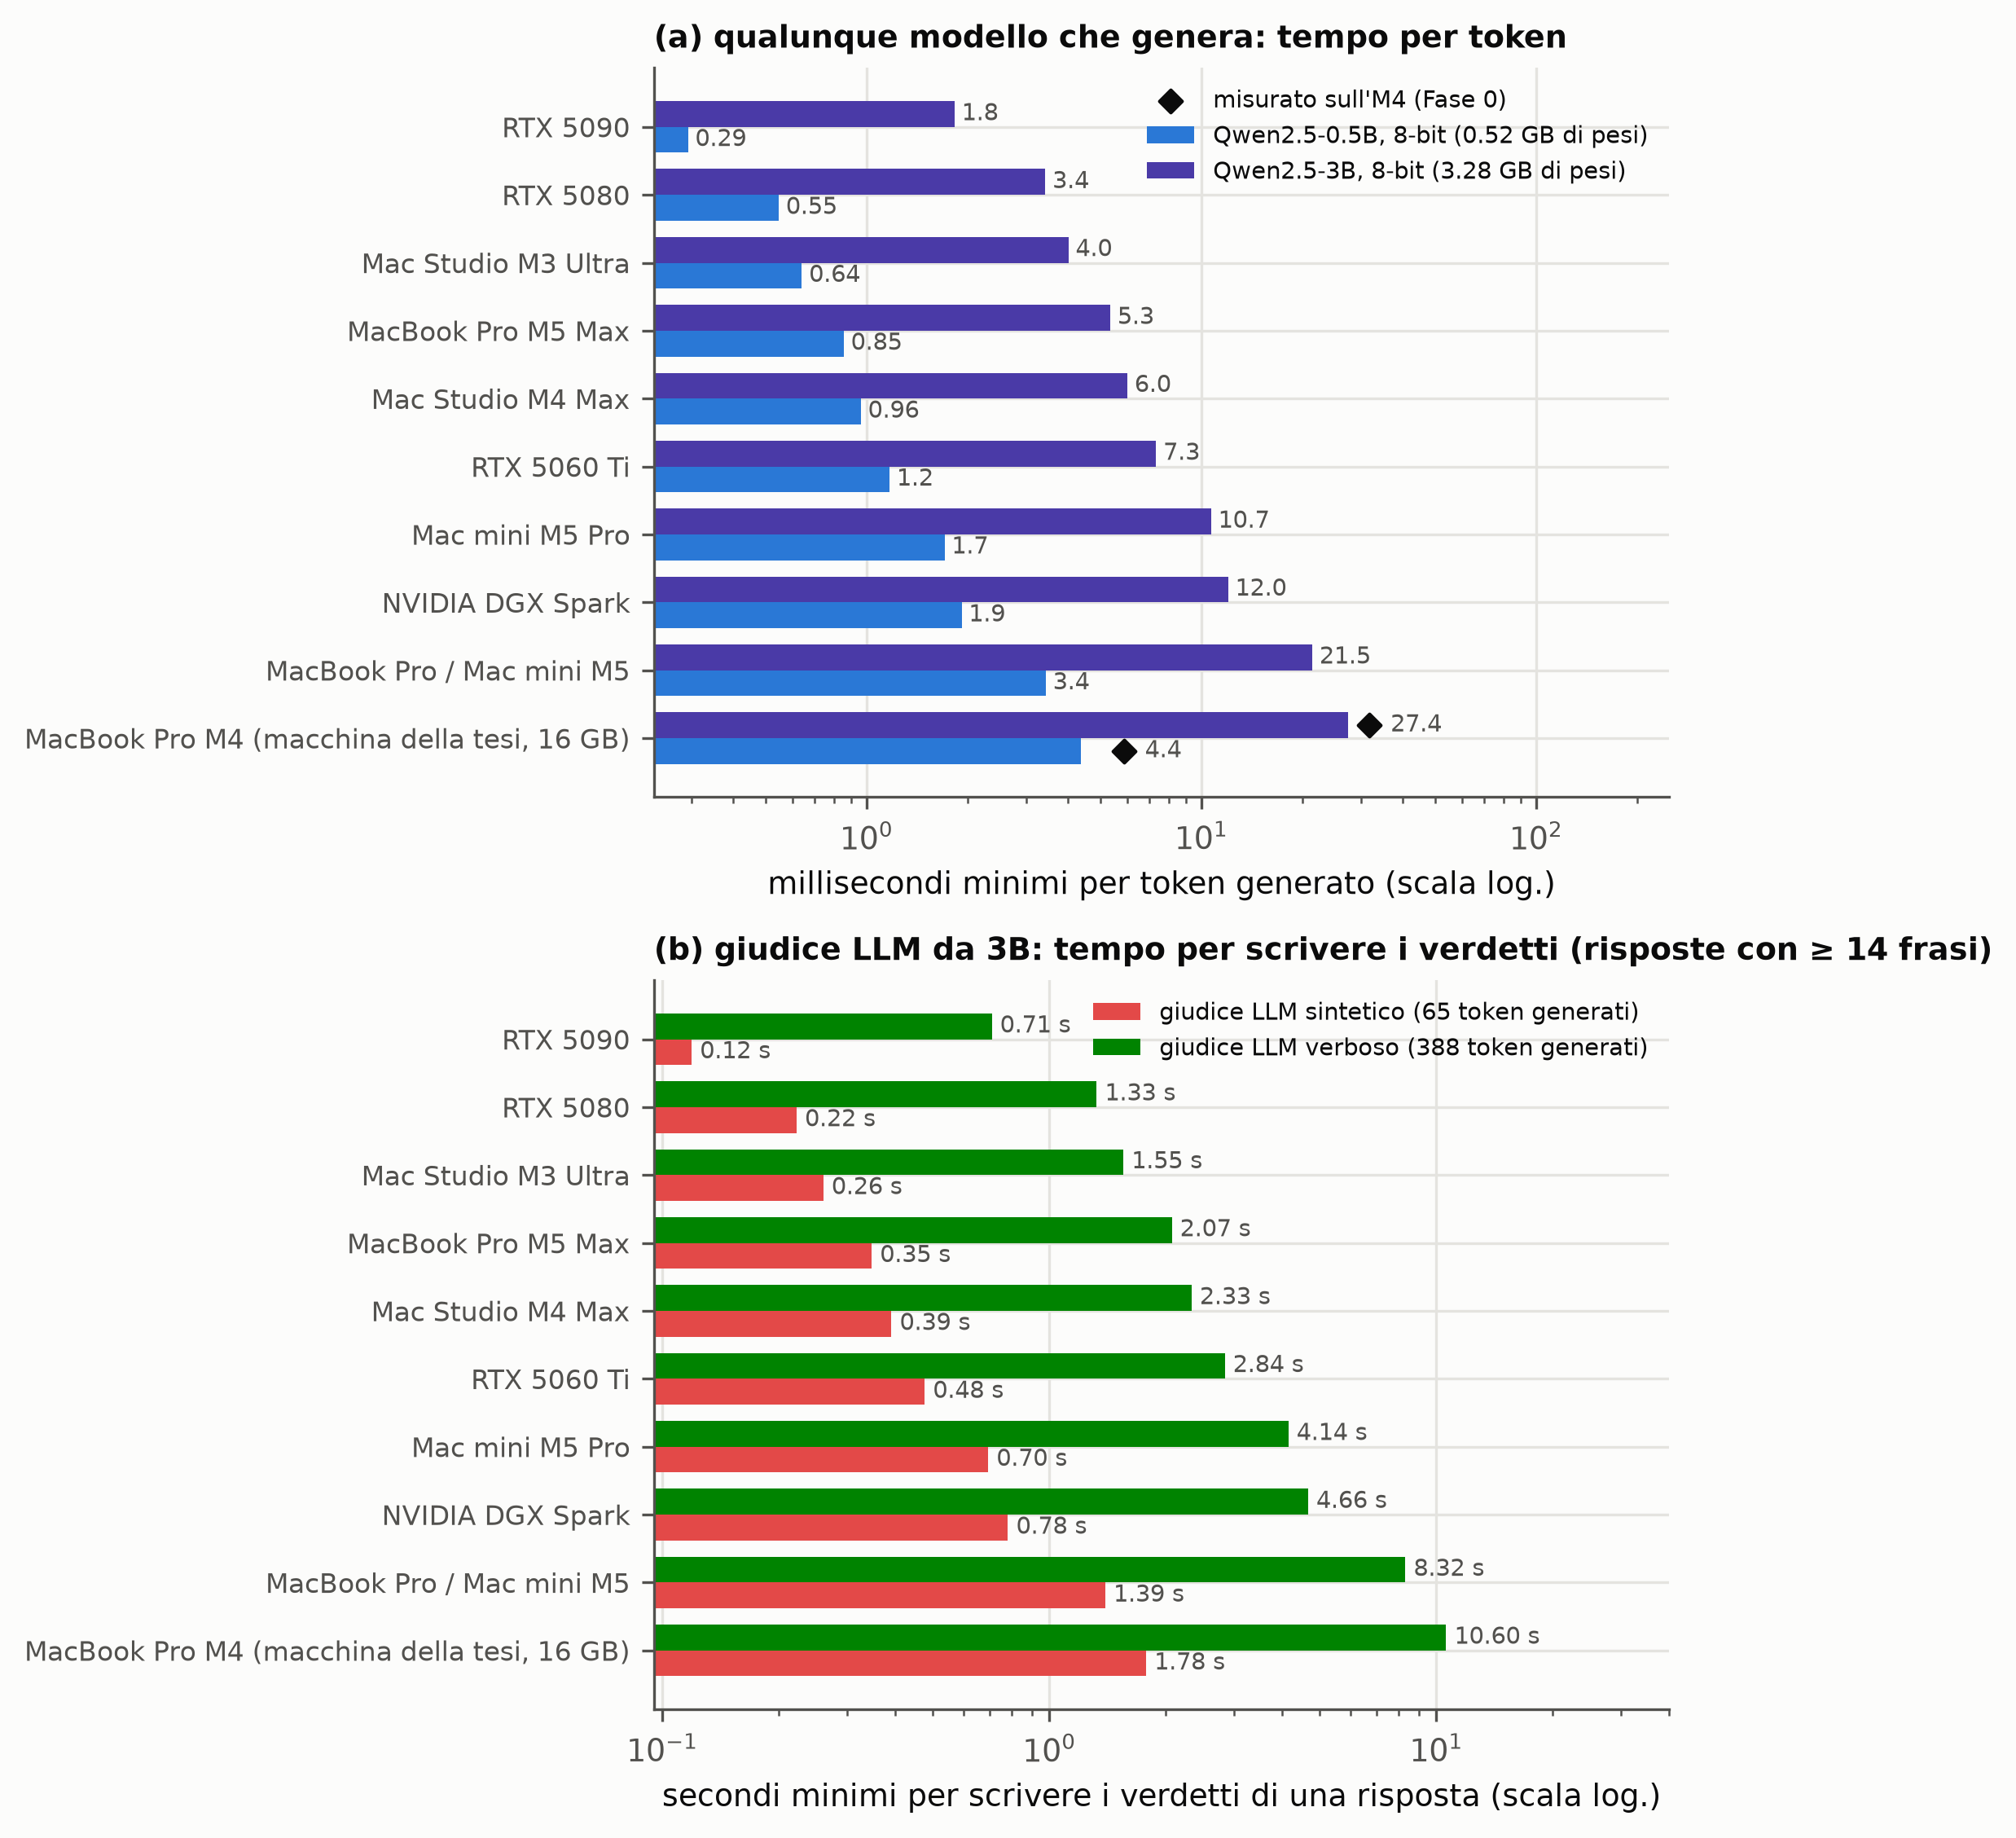
\includegraphics[width=\textwidth]{images/locality/decode_cost_by_hardware.png}
\caption{Limiti inferiori al costo della generazione di testo su ciascuna classe di hardware locale, calcolati come byte
dei pesi divisi per la banda dichiarata dal produttore (una richiesta alla volta; KV cache trascurata). (a) Tempo per
token generato con i due modelli base di GroundOne a 8 bit; rombi: tempo di decoding misurato sulla macchina della tesi.
(b) Tempo minimo che un giudice generativo da 3B impiega soltanto per scrivere i verdetti di una risposta di quattordici o
più frasi (mediana dei token generati nel protocollo di latenza). Un System One non genera alcun token, quindi per esso
entrambi i costi sono nulli su ogni macchina.}
\label{fig:local-floor}
\end{figure}

\section{Runtime e quantizzazione}
\label{sec:local-software}

\subsection{Runtime}
\label{sec:local-runtimes}

Il software per l'inferenza locale è maturato rapidamente. llama.cpp offre inferenza in C e C++ senza dipendenze
esterne, con quantizzazione e supporto per la maggior parte degli acceleratori consumer~\cite{llamacpp}. Ha inoltre
definito il formato GGUF, che raccoglie in un unico file il modello quantizzato e tutto ciò che serve per usarlo, come
il tokenizer e il formato delle conversazioni. Strumenti come Ollama e LM Studio si basano su di esso e riducono a un
solo comando lo scaricamento e l'avvio di un modello. MLX è un framework di calcolo progettato da Apple per la memoria
unificata dei propri processori, con un'interfaccia vicina a NumPy~\cite{mlx2023}. Il suo pacchetto per modelli
linguistici supporta la quantizzazione e il fine-tuning con LoRA direttamente sul dispositivo~\cite{mlxlm}, ed è il
runtime usato in tutta questa tesi.

Il runtime conta quanto il chip. Un confronto tra cinque runtime sulla stessa macchina Apple riporta velocità di decoding
che differiscono di oltre un ordine di grandezza, con MLX e MLC-LLM in cima e il backend Metal generico di PyTorch in
fondo~\cite{rajesh2025apple}; i numeri dello studio non sono del tutto coerenti tra loro e vanno letti come indicativi,
ma la dispersione è abbastanza ampia da resistere all'incertezza. Sugli smartphone, una valutazione di diversi runtime e
dispositivi rileva grandi differenze di velocità, energia e comportamento termico sia tra runtime sia tra
dispositivi~\cite{laskaridis2024melting}.

\subsection{Motori di inferenza specializzati}
\label{sec:local-engines}

Accanto ai runtime generali è comparsa, nel 2026, una seconda famiglia di software: motori di inferenza scritti per pochi
modelli, che rinunciano alla generalità per spingere più in là i limiti di memoria descritti nella
Sezione~\ref{sec:bg-inference}. DwarfStar (ds4), sviluppato da Salvatore Sanfilippo, è un motore nativo ottimizzato per
alcuni grandi modelli open-weight, a partire da DeepSeek V4 Flash, e pensato per Mac con almeno 96\,GB di memoria, per il
DGX Spark e per le macchine Strix Halo~\cite{antirez2026ds4}. Due sue scelte riguardano da vicino questa tesi. La prima è
una KV cache salvata su disco: una conversazione già letta si può riprendere senza rifare il prefill, che su modelli di
queste dimensioni è la parte più costosa di una richiesta lunga. La seconda è la lettura dei pesi direttamente dall'SSD,
che consente di eseguire modelli più grandi della memoria disponibile, al prezzo della velocità.

Colibri porta questa seconda idea all'estremo~\cite{justvugg2026colibri}. Sfrutta il fatto che un modello
mixture-of-experts usa per ogni token solo una piccola parte dei propri pesi: tiene in memoria la parte sempre attiva e
legge gli esperti dal disco quando il router li richiede. In questo modo GLM-5.2, un modello da 744 miliardi di
parametri, gira su un laptop con 25\,GB di memoria. Il prezzo è quello previsto dal modello di costo: la banda di un SSD
è di pochi gigabyte al secondo, molto inferiore a quella della memoria, e secondo gli autori la generazione scende a
0.05--0.1 token al secondo a freddo su quel laptop e a 1.83 token al secondo su una macchina Strix Halo da
128\,GB~\cite{justvugg2026colibri}. È la stessa idea di LLM in a flash~\cite{alizadeh2024flash}, applicata ai modelli a
esperti: la capacità di memoria smette di essere un limite rigido e si trasforma in un limite di banda, ancora più severo. La
Figura~\ref{fig:local-ssd} illustra il meccanismo.

\begin{figure}[!htbp]
\centering
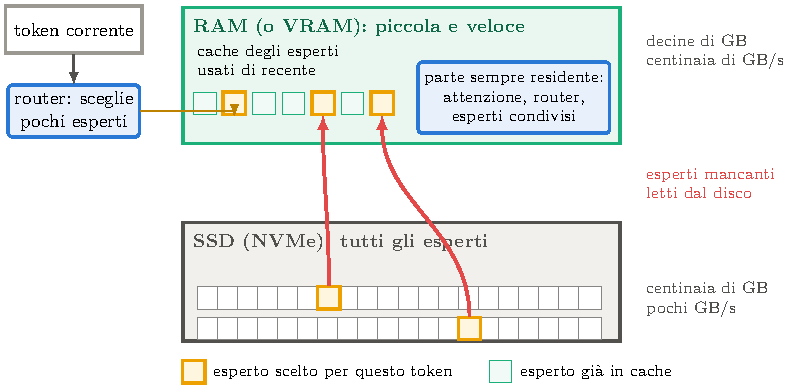
\includegraphics[width=\textwidth]{images/diagrams/ssd_streaming_tikz.pdf}
\caption{Lo streaming degli esperti dall'SSD in un motore come Colibri. In memoria restano la parte del modello usata da
ogni token (attenzione, router, esperti condivisi) e una cache degli esperti usati di recente; tutti gli esperti stanno
sull'SSD. Per ogni token il router sceglie pochi esperti: quelli già in cache si usano subito, quelli mancanti si leggono
dal disco, con una banda di pochi gigabyte al secondo. Per esempio, GLM-5.2 tiene residenti circa 10\,GB e lascia
sul disco circa 429\,GB di pesi~\cite{justvugg2026colibri}. Lo schema non è in scala.}
\label{fig:local-ssd}
\end{figure}

Colibri interessa questa tesi anche per un secondo motivo. Espone la stessa interfaccia System One di Jev, con la quale
qualunque modello che esegue risponde a domande chiuse leggendo la probabilità di ciascuna opzione invece di generare la
risposta, e include in modo nativo tre decision model: Laya, GLiNER2.5-Decide e Clef~\cite{justvugg2026colibri}. Gli
autori riportano che, con Qwen3.6, quattro domande sullo stesso documento ricevono risposta 5.7 volte più velocemente che
generando le stesse risposte sulla stessa CPU. Si tratta di una misura dichiarata dal progetto e non verificata in questa
tesi, ottenuta con modello e hardware diversi, ma va nella stessa direzione dei risultati del
Capitolo~\ref{sec:results}. Che un motore pensato per eseguire modelli enormi su hardware modesto adotti la lettura delle
decisioni come modalità di prima classe conferma che l'idea del System One si sta diffondendo proprio dove generare costa
di più.

\subsection{Quantizzazione}
\label{sec:local-quantisation}

La quantizzazione memorizza i pesi con meno bit dei 16 usati in addestramento. Sull'hardware locale serve a due scopi
contemporaneamente: il modello occupa meno memoria e il decoding diventa più veloce, perché il suo tempo è dominato dalla
lettura dei pesi. La Tabella~\ref{tab:local-quant} riassume i metodi che hanno segnato il campo.

\begin{table}[htbp]
\centering
\caption{Metodi di quantizzazione dei pesi per i modelli linguistici.}
\label{tab:local-quant}
\small
\begin{tabularx}{\textwidth}{@{}lXl@{}}
\toprule
Metodo & Idea e risultato principale & Fonte \\
\midrule
LLM.int8() & Pesi e attivazioni a 8 bit; le poche dimensioni con valori anomali molto grandi (outlier) restano a 16 bit. Nessuna
perdita fino a 175B parametri; fa risparmiare memoria ma non accelera i modelli piccoli & \cite{dettmers2022llmint8} \\
GPTQ & Pesi a 3--4 bit, quantizzati strato per strato stimando quanto ogni peso influisca sull'errore. OPT-175B a 4 bit
perde 0.03 di perplexity\footnote{La \emph{perplexity} misura quanto un modello predice bene un testo: più è bassa,
meno il modello è ``sorpreso'' dalle parole che incontra.}; i modelli piccoli perdono di più; decoding 3.2--4.5$\times$ più veloce grazie alla banda & \cite{frantar2023gptq} \\
AWQ & Pesi a 4 bit; l'1\,\% di canali più importanti, individuato dall'ampiezza delle attivazioni, è protetto tramite
scalatura. Robusto rispetto ai dati di calibrazione; pensato per l'uso sul dispositivo & \cite{lin2024awq} \\
GGUF k-quant & Formati a blocchi da 2 a 8 bit di llama.cpp, standard di fatto per la distribuzione consumer & \cite{llamacpp} \\
MLX affine & Pesi a 4 o 8 bit con una scala e un bias per gruppo di 64; supporta l'addestramento LoRA sul modello
quantizzato (usato in questa tesi) & \cite{mlxlm} \\
QLoRA & Modello base a 4 bit in formato normal float con adapter a 16 bit, per il fine-tuning con memoria limitata &
\cite{dettmers2023qlora} \\
\bottomrule
\end{tabularx}
\end{table}

Due risultati di questa letteratura contano per la tesi. Il primo è che la quantizzazione aiuta la fase limitata dalla
banda. GPTQ attribuisce interamente i propri speed-up ai prodotti matrice-vettore del decoding e dichiara di non ottenere
alcuna riduzione del calcolo~\cite{frantar2023gptq}; AWQ illustra lo stesso punto con un roofline: su una scheda grafica
desktop, un prefill di 200 token richiede 10 millisecondi, mentre generarne 20 ne richiede 310~\cite{lin2024awq}. Ridurre
i bit dei pesi accelera quindi un modello che genera molto più di uno che si limita a leggere. Il secondo è che i modelli
piccoli sono più fragili. GPTQ perde molta più accuratezza a 4 bit su un modello da 1.3 miliardi di parametri che su uno
da 175 miliardi, e sugli smartphone i modelli da tre miliardi di parametri o meno diventano inutilizzabili a 3
bit~\cite{frantar2023gptq,laskaridis2024melting}. LLM.int8() mostra che un pugno di feature outlier controlla una quota
rilevante della massa di probabilità dell'attenzione~\cite{dettmers2022llmint8}. Per un modello il cui output è una
probabilità da calibrare, e non un testo che deve soltanto risultare scorrevole, queste osservazioni suggeriscono una
precisione prudente: GroundOne usa pesi a 8 bit.

\subsection{Generare più in fretta senza generare meno}
\label{sec:local-speculative}

Una diversa famiglia di metodi accelera la generazione senza modificare il modello. Nello speculative decoding un piccolo
modello bozza propone diversi token, e il modello grande li verifica tutti in un unico forward pass, accettando il
prefisso più lungo che avrebbe prodotto esso stesso; l'output è identico a quello del modello grande, e lo speed-up
arriva a due-tre volte~\cite{leviathan2023speculative}. Il metodo è utile per qualunque sistema debba generare, ma non
cambia la natura del costo: ogni token accettato richiede comunque un forward pass del modello grande, e la quantità
totale di calcolo aumenta~\cite{leviathan2023speculative}. Rende la scrittura più economica, non gratuita.

\section{Energia}
\label{sec:local-energy}

Su un dispositivo a batteria l'energia è una proprietà del metodo e non soltanto dell'hardware. Misure su hardware da
datacenter mostrano che l'energia di una richiesta cresce con il numero di token generati e dipende fortemente dalla
dimensione del modello e dal task~\cite{samsi2023words,luccioni2024power}. Sugli smartphone, un modello da 3 miliardi di
parametri a 4 bit spende tra 0.58 e 0.76 joule per token generato, con una potenza sostenuta intorno ai 14\,W e
temperature superficiali vicine ai 48\,\textdegree C~\cite{laskaridis2024melting}; una regola empirica tratta dai lavori
sui modelli piccoli stima il costo in circa 0.1 joule per token generato per ogni miliardo di
parametri~\cite{liu2024mobilellm}. Spostare il prefill sulla NPU di uno smartphone ne riduce l'energia di 1.9--4.3 volte
rispetto all'unità grafica~\cite{xu2025npu}.

La distinzione tra le due fasi vale anche per la potenza. Il prefill tiene occupate le unità aritmetiche e assorbe più
potenza; il decoding attende la memoria e assorbe meno potenza, ma per molto più tempo~\cite{patel2024splitwise}. Un
metodo che fa risparmiare tempo fa quindi risparmiare anche energia, ma in misura minore, e il Capitolo~\ref{sec:results}
misura proprio questo effetto: GroundOne spende 5.5 joule per risposta lunga con il modello da 0.5B e 33 con il 3B, meno
di qualunque giudice generativo della stessa dimensione, ma con un vantaggio inferiore a quello sul tempo
(Sezione~\ref{sec:results-energy}).

\section{Conseguenze per la verifica sul dispositivo}
\label{sec:local-verification}

Il capitolo si può ora riassumere in un'unica osservazione: su un dispositivo locale, che serve una richiesta alla
volta, leggere un token costa molto meno che scriverne uno, quattordici-sedici volte meno sulla macchina della tesi
(Sezioni~\ref{sec:local-phases}--\ref{sec:local-floor}), e le generazioni più recenti di hardware accelerano la lettura
molto più della scrittura (Sezione~\ref{sec:local-asymmetry}). Ne discende una conseguenza diretta per un verificatore che gira
accanto al generatore.

Un giudice generativo verifica una risposta leggendo il documento e la risposta e poi scrivendo i propri verdetti. Paga
un prefill, come ogni metodo che legge il documento, e poi un passo di decoding per ogni token che scrive. Nel protocollo
di latenza di questa tesi (Sezione~\ref{sec:results-latency}), per una risposta di quattordici o più frasi un giudice
sintetico da 3B scrive in mediana 65 token, e uno verboso, che motiva ogni verdetto, ne scrive 388. Il limite inferiore
della Sezione~\ref{sec:local-floor} traduce questi conteggi in un tempo minimo che nessuna implementazione può battere
(Figura~\ref{fig:local-floor}b): sulla macchina della tesi, almeno 1.8 secondi per il giudice sintetico e 10.6 per quello
verboso, oltre al prefill; persino sulla scheda grafica più veloce, 0.12 e 0.71 secondi.

Un System One elimina del tutto questo termine. Legge il documento e la risposta una sola volta e prende ogni decisione
dai logit calcolati durante quell'unica lettura, quindi il suo costo coincide con il solo prefill: la fase limitata dal
calcolo, quella che l'hardware locale esegue bene e che il nuovo hardware accelera di più. Il suo vantaggio su un giudice
non è quindi una proprietà di una particolare macchina, ma della struttura dei costi dell'inferenza locale, ed è massimo
proprio dove l'inferenza è locale. La località, che a prima vista è soltanto un vincolo sulla dimensione del modello,
diventa la ragione per cui il progetto conta.

Da questo capitolo discendono tre requisiti per il verificatore, che guidano il metodo del Capitolo~\ref{sec:method}.
Non deve generare alcun token, così che il suo costo sia un singolo prefill. Deve usare un modello abbastanza piccolo da
condividere una macchina da 16\,GB con un generatore e un retriever, quantizzato in modo prudente perché il suo output è
una probabilità. E deve leggere le proprie decisioni dai logit, che solo un modello locale espone, così che possano essere
calibrate.
